\documentclass[english]{article}
%    qcircuit version 2.6.0
%    Contributors: Steve Flammia, Bryan Eastin, Travis Scholten
%    This program is free software; you can redistribute it and/or modify
%    it under the terms of the GNU General Public License as published by
%    the Free Software Foundation; either version 2 of the License, or
%    (at your option) any later version.
%
%    This program is distributed in the hope that it will be useful,
%    but WITHOUT ANY WARRANTY; without even the implied warranty of
%    MERCHANTABILITY or FITNESS FOR A PARTICULAR PURPOSE.  See the
%    GNU General Public License for more details.
%
%    You should have received a copy of the GNU General Public License
%    along with this program; if not, write to the Free Software
%    Foundation, Inc., 59 Temple Place, Suite 330, Boston, MA  02111-1307  USA

% Thanks to the Xy-pic guys, Kristoffer H Rose, Ross Moore, and Daniel Müllner,
% for their help in making Qcircuit work with Xy-pic version 3.8.  
% Thanks also to Dave Clader, Andrew Childs, Rafael Possignolo, Tyson Williams,
% Sergio Boixo, Cris Moore, Jonas Anderson, and Stephan Mertens for helping us test 
% and/or develop the new version.
\ProvidesPackage{qcircuit}[2018/08/14]
\RequirePackage{xy}

\DeclareOption{braket}{
    \newcommand{\bra}[1]{\ensuremath{\left\langle{#1}\right\vert}}
    \newcommand{\ket}[1]{\ensuremath{\left\vert{#1}\right\rangle}}
    }

\DeclareOption{qm}{
    \newcommand{\ip}[2]{\ensuremath{\left\langle{#1}\middle\vert{#2}\right\rangle}}
    \newcommand{\melem}[3]{\ensuremath{\left\langle{#1}\middle\vert{#2}\middle\vert{#3}\right\rangle}}
    \newcommand{\expval}[1]{\ensuremath{\left\langle #1 \right\rangle}}
    \newcommand{\op}[2]{\ensuremath{\left\vert{#1}\middle\rangle\middle\langle{#2}\right\vert}}
}

\ProcessOptions\relax

\xyoption{matrix}
\xyoption{frame}
\xyoption{arrow}
\xyoption{arc}

\usepackage{ifpdf}
\ifpdf
\else
\PackageWarningNoLine{Qcircuit}{qcircuit is not loading in PDF mode. Activating all Xy-pic features to compensate. If you wish to use specific drivers for Xy-pic, you must modify the code in qcircuit.sty}
%    The following option loads all the features in Xy-pic. This
%    this is included as work-around to ensure documents compile
%    images correctly when using XeLaTeX.
\xyoption{all}
\fi

% The following resets Xy-pic matrix alignment to the pre-3.8 default, as
% required by Qcircuit.
\entrymodifiers={!C\entrybox}

\newcommand{\qw}[1][-1]{\ar @{-} [0,#1]}
    % Defines a wire that connects horizontally.  By default it connects to the object on the left of the current object.
    % WARNING: Wire commands must appear after the gate in any given entry.
\newcommand{\qwx}[1][-1]{\ar @{-} [#1,0]}
    % Defines a wire that connects vertically.  By default it connects to the object above the current object.
    % WARNING: Wire commands must appear after the gate in any given entry.
\newcommand{\qwa}[1][-1]{\ar @{<-} [0,#1]}
    % Defines a wire that connects horizontally with an arrow.  By default it makes an end wire with an arrow indicating the end of the circuit.
    % WARNING: Wire commands must appear after the gate in any given entry.
\newcommand{\cw}[1][-1]{\ar @{=} [0,#1]}
    % Defines a classical wire that connects horizontally.  By default it connects to the object on the left of the current object.
    % WARNING: Wire commands must appear after the gate in any given entry.
\newcommand{\cwx}[1][-1]{\ar @{=} [#1,0]}
    % Defines a classical wire that connects vertically.  By default it connects to the object above the current object.
    % WARNING: Wire commands must appear after the gate in any given entry.
\newcommand{\cwa}[1][-1]{\ar @{<=} [0,#1]}
    % Defines a classical wire that connects horizontally with an arrow.  By default it makes an end wire with an arrow indicating the end of the circuit.
    % WARNING: Wire commands must appear after the gate in any given entry.
\newcommand{\cds}[2]{*+<1em,.9em>{\hphantom{#2}} \POS [0,0].[#1,0]="e",!C *{#2};"e"+ R \qw}
    % Allows the insertion of text without a box and exands circuit around this text.
    % This is useful for such things as ... to indicate a generalized circuit.
\newcommand{\barrier}[2][-0.95em]{\ar @{--}[#2,1]+<#1, -1em>;[0,1]+<#1, 1em>}
    % Defines a barrier that is represented by a horizontal dashed line.
    % It takes a a single argument to specify how many bits to cover
    % To center the barrier between gates you can adjust the horizontal offset
    % with an optional second parameter. This is the horizontal offset in em.
    % It defaults to -0.95em
    % WARNING: Be sure to place the barrier on the topmost bit it covers, it only propogates downwards
\newcommand{\gate}[1]{*+<.6em>{#1} \POS ="i","i"+UR;"i"+UL **\dir{-};"i"+DL **\dir{-};"i"+DR **\dir{-};"i"+UR **\dir{-},"i" \qw}
    % Boxes the argument, making a gate.
\newcommand{\sgate}[2]{\gate{#1}  \qwx[#2]}
    % Creates a gate and a qwx wire going #2 spots below, for a gate split over
    % non-adjacent rows
\newcommand{\meter}{*=<1.8em,1.4em>{\xy ="j","j"-<.778em,.322em>;{"j"+<.778em,-.322em> \ellipse ur,_{}},"j"-<0em,.4em>;p+<.5em,.9em> **\dir{-},"j"+<2.2em,2.2em>*{},"j"-<2.2em,2.2em>*{} \endxy} \POS ="i","i"+UR;"i"+UL **\dir{-};"i"+DL **\dir{-};"i"+DR **\dir{-};"i"+UR **\dir{-},"i" \qw}
    % Inserts a measurement meter.
    % In case you're wondering, the constants .778em and .322em specify
    % one quarter of a circle with radius 1.1em.
    % The points added at + and - <2.2em,2.2em> are there to strech the
    % canvas, ensuring that the size is unaffected by erratic spacing issues
    % with the arc.
\newcommand{\metersymb}{\xy ="j","j"-<.778em,.322em>;{"j"+<.778em,-.322em> \ellipse ur,_{}},"j"-<0em,.4em>;p+<.5em,.9em> **\dir{-},"j"+<2.2em,2.2em>*{},"j"-<2.2em,2.2em>*{} \endxy}
    % A longer meter
\newcommand{\meterB}[1]{*=<1.8em,2.6em>{\xy 0;<0em,-.8em>:
0*{\begingroup
\everymath{\scriptstyle}
\tiny #1 \endgroup},<0em,.7em>*{\xy ="j","j"-<.778em,-.322em>;{"j"+<.778em,.322em> \ellipse ur,_{}},"j"-<0em,-.2em>;p+<.5em,.9em> **\dir{-},"j"+<2.2em,2.2em>*{},"j"-<2.2em,2.2em>*{} \endxy} 
\endxy} \POS ="i","i"+UR;"i"+UL **\dir{-};"i"+DL **\dir{-};"i"+DR **\dir{-};"i"+UR **\dir{-},"i" \qw}
    % A meter that allows for a measurement operator to be added below
\newcommand{\smeterB}[2]{\meterB{#1} \qwx[#2] \qw}
    % A split meter that allows for a measurement operator to be split over non-
    % adjacent rows
\newcommand{\measure}[1]{*+[F-:<.9em>]{#1} \qw}
    % Inserts a measurement bubble with user defined text.
\newcommand{\measuretab}[1]{*{\xy*+<.6em>{#1}="e";"e"+UL;"e"+UR **\dir{-};"e"+DR **\dir{-};"e"+DL **\dir{-};"e"+LC-<.5em,0em> **\dir{-};"e"+UL **\dir{-} \endxy} \qw}
    % Inserts a measurement tab with user defined text.
\newcommand{\measureD}[1]{*{\xy*+=<0em,.1em>{#1}="e";"e"+UR+<0em,.25em>;"e"+UL+<-.5em,.25em> **\dir{-};"e"+DL+<-.5em,-.25em> **\dir{-};"e"+DR+<0em,-.25em> **\dir{-};{"e"+UR+<0em,.25em>\ellipse^{}};"e"+C:,+(0,1)*{} \endxy} \qw}
    % Inserts a D-shaped measurement gate with user defined text.
\newcommand{\multimeasure}[2]{*+<1em,.9em>{\hphantom{#2}} \qw \POS[0,0].[#1,0];p !C *{#2},p \drop\frm<.9em>{-}}
    % Draws a multiple qubit measurement bubble starting at the current position and spanning #1 additional gates below.
    % #2 gives the label for the gate.
    % You must use an argument of the same width as #2 in \ghost for the wires to connect properly on the lower lines.
\newcommand{\multimeasureD}[2]{*+<1em,.9em>{\hphantom{#2}} \POS [0,0]="i",[0,0].[#1,0]="e",!C *{#2},"e"+UR-<.8em,0em>;"e"+UL **\dir{-};"e"+DL **\dir{-};"e"+DR+<-.8em,0em> **\dir{-};{"e"+DR+<0em,.8em>\ellipse^{}};"e"+UR+<0em,-.8em> **\dir{-};{"e"+UR-<.8em,0em>\ellipse^{}},"i" \qw}
    % Draws a multiple qubit D-shaped measurement gate starting at the current position and spanning #1 additional gates below.
    % #2 gives the label for the gate.
    % You must use an argument of the same width as #2 in \ghost for the wires to connect properly on the lower lines.
\newcommand{\control}{*!<0em,.025em>-=-<.2em>{\bullet}}
    % Inserts an unconnected control.
\newcommand{\controlo}{*+<.01em>{\xy -<.095em>*\xycircle<.19em>{} \endxy}}
    % Inserts a unconnected control-on-0.
\newcommand{\ctrl}[1]{\control \qwx[#1] \qw}
    % Inserts a control and connects it to the object #1 wires below.
\newcommand{\ctrlo}[1]{\controlo \qwx[#1] \qw}
    % Inserts a control-on-0 and connects it to the object #1 wires below.
\newcommand{\cctrl}[1]{\control \cwx[#1] \cw}
    % Inserts a classical control and connects it to the object #1 wires below. 
\newcommand{\cctrlo}[1]{\controlo \cwx[#1] \cw}
    % Inserts a classical control-on-0 and connects it to the object #1 wires below.    
\newcommand{\targ}{*+<.02em,.02em>{\xy ="i","i"-<.39em,0em>;"i"+<.39em,0em> **\dir{-}, "i"-<0em,.39em>;"i"+<0em,.39em> **\dir{-},"i"*\xycircle<.4em>{} \endxy} \qw}
    % Inserts a CNOT target.
\newcommand{\qswap}{*=<0em>{\times} \qw}
    % Inserts half a swap gate.
    % Must be connected to the other swap with \qwx.
\newcommand{\multigate}[2]{*+<1em,.9em>{\hphantom{#2}} \POS [0,0]="i",[0,0].[#1,0]="e",!C *{#2},"e"+UR;"e"+UL **\dir{-};"e"+DL **\dir{-};"e"+DR **\dir{-};"e"+UR **\dir{-},"i" \qw}
    % Draws a multiple qubit gate starting at the current position and spanning #1 additional gates below.
    % #2 gives the label for the gate.
    % You must use an argument of the same width as #2 in \ghost for the wires to connect properly on the lower lines.
\newcommand{\ghost}[1]{*+<1em,.9em>{\hphantom{#1}} \qw}
    % Leaves space for \multigate on wires other than the one on which \multigate appears.  Without this command wires will cross your gate.
    % #1 should match the second argument in the corresponding \multigate.
\newcommand{\cghost}[1]{*+<1em,.9em>{\hphantom{#1}} \cw}
    % Same as ghost but with a classical incoming wire.
\newcommand{\nghost}[1]{*+<1em,.9em>{\hphantom{#1}}}
    % Same as ghost but with no incoming wire.
\newcommand{\push}[1]{*{#1}}
    % Inserts #1, overriding the default that causes entries to have zero size.  This command takes the place of a gate.
    % Like a gate, it must precede any wire commands.
    % \push is useful for forcing columns apart.
    % NOTE: It might be useful to know that a gate is about 1.3 times the height of its contents.  I.e. \gate{M} is 1.3em tall.
    % WARNING: \push must appear before any wire commands and may not appear in an entry with a gate or label.
\newcommand{\gategroup}[6]{\POS"#1,#2"."#3,#2"."#1,#4"."#3,#4"!C*+<#5>\frm{#6}}
    % Constructs a box or bracket enclosing the square block spanning rows #1-#3 and columns=#2-#4.
    % The block is given a margin #5/2, so #5 should be a valid length.
    % #6 can take the following arguments -- or . or _\} or ^\} or \{ or \} or _) or ^) or ( or ) where the first two options yield dashed and
    % dotted boxes respectively, and the last eight options yield bottom, top, left, and right braces of the curly or normal variety.  See the Xy-pic reference manual for more options.
    % \gategroup can appear at the end of any gate entry, but it's good form to pick either the last entry or one of the corner gates.
    % BUG: \gategroup uses the four corner gates to determine the size of the bounding box.  Other gates may stick out of that box.  See \prop.
\newcommand{\inputgroupv}[5]{\POS"#1,1"."#2,1"."#1,1"."#2,1"!C*+<#3>\frm{\{}, \POS"#1,1"."#2,1"."#1,1"."#2,1"*!C!<1.7em,#4>=<0em>{#5}}
    % Constructs an input group with label #5 and a grouping { from rows #1 to #2 with #3 and #4 controlling the spacing
\newcommand{\inputgroup}[4]{\POS"#1,1"."#2,1"."#1,1"."#2,1", \POS"#1,1"."#2,1"."#1,1"."#2,1"*!C!<1em,#3>=<0em>{#4}}
    % Constructs an input group with label #4 from rows #1 to #2 with #3 controlling the spacing
\newcommand{\inputgrouph}[5]{\POS"#1,1"."#2,1"."#1,1"."#2,1", \POS"#1,1"."#2,1"."#1,1"."#2,1"*!C!<#5,#3>=<0em>{#4}}
    % Constructs an input group with label #4 and a grouping /vdots from rows #1 to #2 with #3 and #5 controlling the spacing
\newcommand{\rstick}[1]{*!L!<-.5em,0em>=<0em>{#1}}
    % Centers the left side of #1 in the cell.  Intended for lining up wire labels.  Note that non-gates have default size zero.
\newcommand{\lstick}[1]{*!R!<.5em,0em>=<0em>{#1}}
    % Centers the right side of #1 in the cell.  Intended for lining up wire labels.  Note that non-gates have default size zero.
\newcommand{\ustick}[1]{*!D!<0em,-.5em>=<0em>{#1}}
    % Centers the bottom of #1 in the cell.  Intended for lining up wire labels.  Note that non-gates have default size zero.
\newcommand{\dstick}[1]{*!U!<0em,.5em>=<0em>{#1}}
    % Centers the top of #1 in the cell.  Intended for lining up wire labels.  Note that non-gates have default size zero.
\newcommand{\Qcircuit}{\xymatrix @*=<0em>}
    % Defines \Qcircuit as an \xymatrix with entries of default size 0em.
\newcommand{\link}[2]{\ar @{-} [#1,#2]}
    % Draws a wire or connecting line to the element #1 rows down and #2 columns forward.
\newcommand{\pureghost}[1]{*+<1em,.9em>{\hphantom{#1}}}
    % Same as \ghost except it omits the wire leading to the left. 

\endinput


% packages
\usepackage[T1]{fontenc}
\usepackage[utf8]{inputenc}
\usepackage{graphicx}
\usepackage{hyperref}
\usepackage{amssymb}
\usepackage{amsmath}
\usepackage[toc,page]{appendix}
\usepackage{listings}
\usepackage{enumitem}
\usepackage{tikz}
\usepackage{braket}

% commands
\newcommand{\sbigotimes}{%
	\mathop{\mathchoice{\textstyle\bigotimes}{\bigotimes}{\bigotimes}{\bigotimes}}%
}
\newcommand{\zeroket}{\begin{pmatrix} 1 \\ 0 \end{pmatrix}}
\newcommand{\oneket}{\begin{pmatrix} 0 \\ 1 \end{pmatrix}}

% settings
\lstset{language=Python}
\lstset{basicstyle=\footnotesize}
\graphicspath{{img/}}

\begin{document}
	\title{An Introduction to Quantum Computing for Computer Scientists, with SAT}
	\author{Francesco Piro}
	\maketitle
	
	\begin{abstract}
		This paper wants to provide the introduction to the quantum computation area with an approach based in particular on coding examples that allow to understand how the physical and mathematical principles introduced are encoded in a quantum circuit. To do so we considered the satisfiability problem as a reference during the entire paper for its importance in the computational theory field in particular with respect to the $\mathcal{N}\mathcal{P}$-complete problems. To conclude the study by showing the complexity enhancements achieved with respect to the classical solver we used Grover's search algorithm to find the solution of the generalized k-SAT problem in quadratic time faster.
	\end{abstract}

	\section*{Introduction}
	\label{sec:introduction}
	Quantum computation is a wide area involving several disciplines that is having always more success in nowadays applications thanks in particular to the development of the technology and its incredible results. Quantum physics' principles are the fundamentals on which the entire theory is based: thanks to their properties, new architectures allow to define devices that can solve classical problems in surprisingly reduced time and space complexities. However we always have a trade-off to consider, in particular now that these technology are still emerging.\\
	
	This paper aims at giving a description for computer scientists of what a quantum computer is and which are its real impacts and advantages with respect to the classical ones. Hence I will try to provide a description of the state of the art of quantum computing with an approach that allows to understand how from the basic principles of quantum mechanics we are able to have an algorithm that is faster with respect to its classic counterpart. In order to do so in the first chapter (\ref{sec:quantumComputing}) I will start with the basic linear algebra needed to study the quantum physics' principles we need to define a quantum computer. The definition of the \emph{quantum computer} is fundamental both to understand how an algorithm is executed but also to have a comparison with the classic Turing machine that allows to determine conclusions about computational complexity (chapter \ref{sec:computationalTheory}). Once the background on quantum computation and computational theory are well consolidated by the reader, the last chapters provide a practical example that is used to prove the speedup for the particular \textbf{satisfiability problem.} I have used an efficient classical solver for the \emph{k-SAT} as I could compare it with my quantum implementation, both realized in python. In the end I provide some important conclusions for quantum computing that I was able to conclude thanks to my study, in particular in the papers listed in the references. \\
	
	The paper follows a structure that allows to define the \textbf{state of the art} of quantum computation by fixing the most important definitions and conclusions as soon as they are encountered in the reading. The most important concepts that this study wants to define are highlighted as numbered conclusions as they can be referred during the following descriptions. Typically to underline complex concepts we used practical examples and when possible, to stick with our aiming public, some snippets of code are shown in order to give additional clarity.
	
	\section{Quantum Computing}
	\label{sec:quantumComputing}
		This chapter aims at providing first the fundamentals needed in order to deal with quantum mechanics and second at defining a quantum computer thanks to the principles previously identified. With the quantum device we will be able to make a comparison with the classical one to understand with examples how the basic operations are realized in order to use them to implement complete algorithms. Further in the chapter, a section is completely dedicated to the main quantum search algorithm that is fundamental to solve the SAT. Also here we will start from a classical version to compare it with its quantum counterpart. All the arguments related in this chapter, together with the ones in the next (\ref{sec:computationalTheory}) are fundamental to give a significant interpretation to the comparison between the classic and quantum implementation of the algorithm able to solve the \textbf{satisfiability problem} (\ref{sec:sat}).
		
		\subsection{Fundamentals}
		\label{sec:fundamentals}
			The study of quantum computers requires the knowledge of the decimal and binary representation of integers, probability notions and in particular linear algebra fundamental definitions like the ones of: \emph{vectors, spaces, bases, linear systems, tensor product...}. In this section are presented the basic concepts needed to face the quantum physics principles that we need in order to realize the quantum computer. 
			
			\subsubsection{Linear Algebra}
			\label{sec:linearAlgebra}
			Basic principles of linear algebra are assumed to be well known by the reader, I want now to remark only the most important operators and definitions that we need in order to face the definition of the following quantum mechanical theorems. The most important notions we want to acquire from this section are: \emph{tensor product, Hilbert space, bra-ket notation}.\\
			
			In order to realize a quantum computer we need to understand how to define a state that is able to contain information that can be used to obtain a certain objective. As we will see in the next section, the state of a quantum device is a quantum state, thus a mathematical model that lives into a specific \emph{vector state} whose dimension depends on the amount of information it needs to encode. Typically, significant states contain information that results from the composition of several spaces combined together thanks to a particular operator called tensor product.
			
			\paragraph{Definition (Tensor Product):} \emph{Given two vector spaces V and W over a field K with bases $e_1,..., e_m$ and
$f_1,..., f_n$ respectively, the tensor product $V \otimes W$ is another vector space over K of dimension
mn. The tensor product space is equipped with a bilinear operation $\otimes : V \times W \rightarrow V \otimes W$. The
vector space $V \otimes W$ has basis $e_i \otimes f_j \forall i = 1,...,m, j = 1,...,n$}. \\
			
			Typically we are going to work with complex Euclidean vector spaces of the form $\mathbb{C}^n$ and, by choosing the standard basis in the origin vector spaces, then the tensor product is nothing more than the Kronecker product.
			
			\paragraph{Definition (Kronecker Product):} \emph{Given $A \in \mathbb{C}^{m\times n}$, $B \in \mathbb{C}^{p\times q}$, the Kronecker product $A \otimes B$ is the matrix $D \in \mathbb{C}^{mp\times nq}$ defined as:}
			\begin{center}
				$
				D = A\otimes B =
				\begin{pmatrix}
				a_{11}B & \cdots & a_{1n}B \\
				a_{21}B & \cdots  & a_{2n}B \\
				\vdots & \vdots & \vdots \\
				a_{m1}B & \cdots & a_{mn}B
				\end{pmatrix}
				$
			\end{center}
		
			Now that we know the notions of vector state and tensor product, we can use them to define an important space (in particular for the SAT problem we are going to study later) called the \textbf{Hilbert space} and denoted with $\mathcal{H}$.
			
			\paragraph{Definition (Hilbert Space):} \emph{Given the complex space $\mathbb{C}$ we define the Hilbert space $\mathcal{H}$ as the (n + 1)-tuple tensor product:}
			\begin{center}
				$
				\mathcal{H} := \sbigotimes_1^{n+1} \mathbb{C}^{2}
				$
			\end{center}
		
			As we said, in the Hilbert space we will carry the discussion of the SAT problem but to understand what the result of this tensor product actually defines we still need to give probably the most important definition. In order to represent a quantum state we use the so called \emph{bra-ket notation} introduced in 1939 by Paul Dirac.
			
			\paragraph{Definition (Dirac/bra-ket Notation):} \emph{Given a complex Euclidean space $\mathbb{S} \equiv \mathbb{C}^{n}$, $|\psi\rangle \in \mathbb{S}$ denotes a column vector, and $\langle\psi| \in \mathbb{S}^{*}$ denotes a row vector that is the conjugate transpose of $|\psi\rangle$, i.i. $\langle\psi| = |\psi\rangle$. The vector $|\psi\rangle$ is also called a ket, while the vector $\langle\psi|$ is also called a bra.} \\
			
			The bra-ket notation allows us to define a quantum state, hence a vector that lives into a particular vector space. Its definition intrinsically defines also the result of combining two states living in the same state with the \textbf{inner product}, straightforwardly obtained from what we have just said: $\langle\psi|\phi\rangle$. This result is fundamental to define spaces that are higher than one only dimension as the Hilbert state presented before. To understand what $\mathcal{H}$ is, we can use two examples where we define the basis of the first two results obtained by doing the tensor product of the complex space $\mathbb{C}^{2}$ with itself. Remember that the basis of a space is the smallest set of linearly independent vectors that can be used to represents all the vectors that belong to that space.
			
			\paragraph{Example 1:} 
			\label{ex:c2}
			\emph{Considering the basic case of $\mathbb{C}^{2}$ the basis can be trivially identified as:}
			\begin{center}
				$|0\rangle = \zeroket \hspace{1cm} |1\rangle = \begin{pmatrix} 0 \\ 1 \end{pmatrix}$
			\end{center}
		
			\paragraph{Example 2:} 
			\label{ex:c4}
			\emph{Considering a single product, thus $\sbigotimes_1^{1} \mathbb{C}^{2} = \mathbb{C}^{2} \otimes \mathbb{C}^{2}$, we obtain the basis by multiplying in all possible ways the vectors of the basis of the previous example. We now have kets of dimension 2, thus vectors with 4 lines and 1 column:}
			\begin{center}
					$
					|00\rangle = |0\rangle \otimes |0\rangle = \zeroket \otimes \zeroket = 
					\begin{pmatrix}
					1\zeroket \vspace{3pt} \\
					0\zeroket
					\end{pmatrix} =
					\begin{pmatrix}
					1 \\ 0 \\ 0 \\ 0
					\end{pmatrix}
					$\vfill
					$
					|01\rangle = |0\rangle \otimes |1\rangle = \zeroket \otimes \oneket = 
					\begin{pmatrix}
					1\oneket \vspace{3pt} \\
					0\oneket
					\end{pmatrix} =
					\begin{pmatrix}
					0 \\ 1 \\ 0 \\ 0
					\end{pmatrix}
					$ \vfill
					$
					|10\rangle = |1\rangle \otimes |0\rangle = \oneket \otimes \zeroket = 
					\begin{pmatrix}
					0\zeroket \vspace{3pt} \\
					1\zeroket
					\end{pmatrix} =
					\begin{pmatrix}
					0 \\ 0 \\ 1 \\ 0
					\end{pmatrix}
					$ \vfill
					$
					|11\rangle = |1\rangle \otimes |1\rangle = \oneket \otimes \oneket = 
					\begin{pmatrix}
					0\oneket \vspace{3pt} \\
					1\oneket
					\end{pmatrix} =
					\begin{pmatrix}
					0 \\ 0 \\ 0 \\ 1
					\end{pmatrix}
					$
			\end{center}
		
			Thanks to these two examples we now know how to generalize the $n + 1$ case and obtain the definition of the Hilbert space we gave before. \\
			
			Before beginning with the quantum physics section where we will start by defining the smallest unit element we use to represent information, the so called \textbf{qubit}, we need to give one further definition. In order to perform operations on qubits we will consider (section \ref{sec:operationsOnQubits}) only a particular family of matrices called unitary matrices. These matrices allow to perform operations on qubits without modifying the basic properties of the quantum state and are defined as follows.
			
			\paragraph{Definition (Unitary Matrix):} \emph{A complex square matrix U is unitary if $U^{*}U = UU^{*} = I$.} \\
			
			Unitary matrices have significant importance in quantum mechanics because they are \textbf{norm-preserving}; this will be fundamental to identify the two main features of quantum operations that can now be summarized as: \emph{by applying a unitary matrix on a quantum state, we obtain a vector whose norm will be preserved}.
						
			\subsubsection{Quantum Physics}
			\label{sec:quantumMechanics}
				Quantum mechanics is a fundamental theory in physics describing the properties of nature. We do not need its entire power for our purpose but, starting from some basic concepts we will exploit the conclusions that are useful to design an algorithm that is faster than its classical counterpart. As we do when we start studying computer science, we want to identify the smallest, most basic element that allows us to represent the information. From a classical point of view we have the \textbf{bit} whose values can be either 1 or 0. From a quantum point of view, instead, we have the \textbf{qubit}, complex variables that can assume values ranging from 0 to 1 (in modulus), identified in a complex space over a surface called the \emph{Block Sphere}.
				
				\paragraph{Definition (Qubit:)} \emph{The qubit is the smallest unit of measurement used to quantify information in quantum computing. It identifies the bit in a superposition, hence both 0 and 1 values are considered. Formally it is a vector of the space $\mathbb{C}^{2}$ represented as a linear combination of the elements contained in its basis (\ref{ex:c2}). A qubit $\psi$, with $\alpha_0,\alpha_1\in\mathbb{C}$, is defined as:}\\
				\begin{center}
					$
					|\psi\rangle = \alpha_0 |0\rangle + \alpha_1 |1\rangle = \alpha_0\zeroket + \alpha_1\oneket
					$
				\end{center}
				
				To understand better the definition of the qubit we now provide its representation in a tridimensional space whose directions are obtained from basic linear algebra principles that are not now relevant. We just need to understand that, thanks to the coefficients $\alpha_0$ and $\alpha_1$ belonging to the complex space $\mathbb{C}$ we are able to consider the basic element of our computation as one of the infinite points that live over the surface of a sphere. We can grasp in this concept a first hint in the advantages that quantum states provide with respect to their classic counterpart.
				
				\paragraph{Definition (Block Sphere):} \emph{The Block Sphere is the geometrical representation of the pure state space of a two-level quantum mechanical system. In other words it represents all the possible vectors that can be obtained by combining the vectors of the basis for a quantum register of 1 qubit.}\\
				
				Consider the following examples to understand how vectors are represented in the Bloch sphere; we present the trivial cases for both $|0\rangle$ and $|1\rangle$ and the respective orthogonal vectors identifying the x and y axes.
	
				\paragraph{Example 3:} \emph{Consider the qubit $\ket{\psi}$, with $\alpha_0,\alpha_1\in\mathbb{C}$, such that: 	$|\psi\rangle = \alpha_0 |0\rangle + \alpha_1 |1\rangle$. (Check code at \ref{c:example3})}
				
				\begin{enumerate}
					\centering
					\begin{figure}[h]
						\begin{minipage}{0.4\textwidth}
							\item $\alpha_0=1, \;\alpha_1=0$
							\centering
							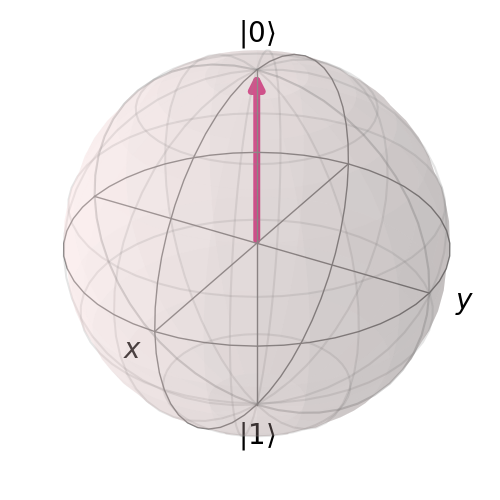
\includegraphics[scale=0.33]{zeroket.png}
							\caption{$|\psi\rangle= |0\rangle$}
						\end{minipage} \hfill
						\begin{minipage}{0.4\textwidth}
							\item $\alpha_0=0, \;\alpha_1=1$
							\centering
							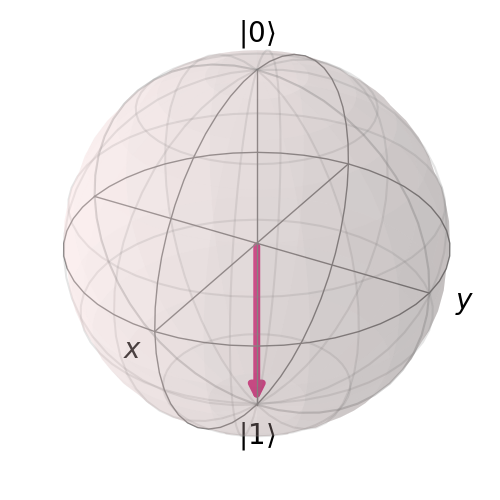
\includegraphics[scale=0.33]{oneket.png}
							\caption{$|\psi\rangle= |1\rangle$}
						\end{minipage}
					\end{figure}
					\begin{figure}[h]
						\begin{minipage}{0.4\textwidth}
							\item $\alpha_0=\frac{1}{\sqrt{2}}, \;\alpha_1=\frac{1}{\sqrt{2}}$
							\centering
							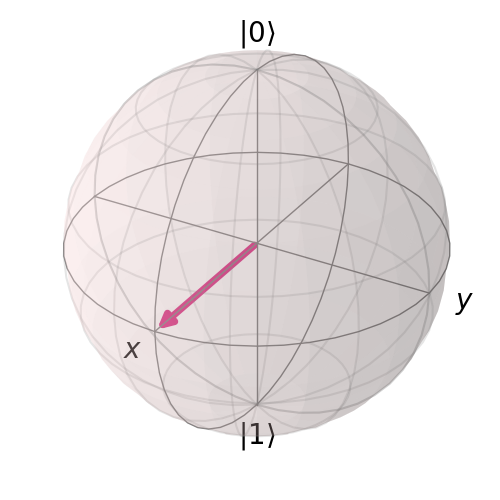
\includegraphics[scale=0.33]{xket.png}
							\caption{$|\psi\rangle = \frac{1}{\sqrt{2}}(|0\rangle+|1\rangle)$}
						\end{minipage} \hfill
						\begin{minipage}{0.4\textwidth}
							\item $\alpha_0=\frac{1}{\sqrt{2}}, \;\alpha_1=\frac{i}{\sqrt{2}}$
							\centering
							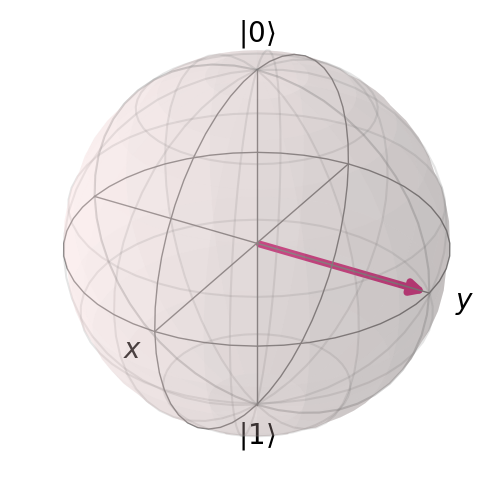
\includegraphics[scale=0.33]{yket.png}
							\caption{$|\psi\rangle = \frac{1}{\sqrt{2}}(|0\rangle+i|1\rangle)$}
						\end{minipage}
					\end{figure}
				\end{enumerate}
			
			Obviously we can also represent vectors that belong to spaces with a higher dimension than 2, in this case we will have their representation over a hypersphere (check the plot\_bloch\_multivector method in the qiskit library). As in classical computer we haver registers, defined as a sequence of bits, in quantum computing we have \emph{quantum-registers} composed of a sequence of qubits. Typically a quantum computer has a single quantum-register made up of qubits (see section \ref{sec:quantumComputer}). It is now important to remark the first conclusion on quantum computing, that derives from the definition of quantum-register that we have just provided. We see that $\sbigotimes_1^{n+1} \mathbb{C}^{2}$ is a $2^{n}$ dimensional space. This is sharp in contrast with what happens for classical registers: given n classical bits, their state is a binary string in $\{0,1\}^{n}$, thus an n-dimensional space. In other words we arrived to the first important conclusion.
			
			\paragraph{Conclusion 1:} \emph{The dimension of the state space of quantum registers grows exponentially in the number of qubits, whereas the dimension of the state space of classical registers grows linearly in the number of bits.}
			
			\subsubsection{Superposition}
			\label{sec:superposition}
				The mathematical definition of the qubit we have just seen is useful to understand the first difference between the representation of a state either in classical or quantum fields. We want now to define from a more physical point of view what means for a qubit to assume both the value 0 and 1. The basic physical principle behind this property is the \emph{Heisenberg uncertainty principle}, but without going too deep in the details let's try to understand it with a simple example. 
				
				\paragraph{Example 4:} \emph{We have seen that bits can assume at a certain time instant one and one value only. Considering now a qubit we could say that it assumes both the values 1 and 0 because its definition is based on Heisenberg's principle, basically stating that particles can assume at the same time different positions. This is a physics principle: electrons can be at the same time in different positions. That is why considering the position 0 and the position 1 we can say that a qubit is situated in both of them. The sad reality is that we do not know the real state of the qubit until we perform a specific operation on it, called measurement, which makes it collapse either to a 0 or a 1 "boring" bit. The following picture tries to illustrate the principle of an electron whose real position is not deterministic until this operation.}
				
				\newpage
				
				\begin{figure}[ht]
					\centering
					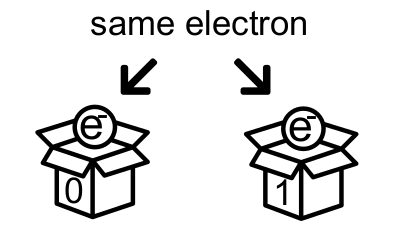
\includegraphics[scale=0.75]{superposition.png}
					\caption{Superposition of the electron}
				\end{figure}
			
				As we may have understood superposition is a very interesting property, also because it can be generalized to the case of n qubits rather than just one. We will se in the implementation of the SAT algorithm how operations on multiple qubits are able to exploit superposition in order to compute the solution of the problem. With this property we can start guessing how algorithms will be run on our quantum computer: from a certain initial state we will perform operations that exploit the indetermination principle over the qubits, thus considering several states at the same time, until the end when performing the measurement will make them collapse to a single string of 1s and 0s which is our result.
			
			\subsubsection{Entanglement}
			\label{sec:entanglement}
				Entanglement is the second main feature of quantum computers that, together with superposition, differentiates them from quantum computers. These are in fact the two main features that are exploited in algorithms to find the solution of a problem. \\
				
				To understand entanglement we start by answering the following question: \\ \\				
				$\underline{What \; do \; we \; gain \; by \; moving \; from \; single \; qubits \; spaces \; to \; multiple \; qubits \; spaces?}$ \\
				
				The answer has two motivations, the first regarding the states representation the second the property of entanglement:
				\begin{enumerate}[label=(\roman*)]
					\item As we described before, also in quantum computing we will need to define registers that contain more than 1 qubit. To do so it suffices to compose a vector of n qubits which identify the state obtained by the result of their quantum product.
					
					\item Linear algebra definitions, in particular for what concerns the tensor products, show that not every state that we consider can be represented as the tensor product of n-qubits. Whenever we have to deal with a state of that kind we will say that the quantum state is entangled.
				\end{enumerate}
			
				More formally the definition of entanglement is the following:
				
				\paragraph{Definition (Entanglement):} \emph{A quantum state $|\psi\rangle \in \sbigotimes_1^{n+1} \mathbb{C}^{2}$ is a product state if it can be expressed as a tensor product $|\psi_0\rangle \otimes |\psi_1\rangle \otimes \cdots \otimes |\psi_n\rangle$ of n 1-qubit states. Otherwise, it is entangled.} \\
				
				To understand better the definition let's consider the simplest example possible: considering a state living in the $\mathbb{C}^4$ complex space we want to check if it is a product state or entangled by looking for two 1-qubit states whose tensor product is the state that we are dealing with. We will see next how the entanglement feature can be used, in particular what happens when 2 qubits are entangled together.
				
				\paragraph{Example 5:} {Consider the following 2-qubit state:
				\begin{align*}
					\frac{1}{2}|00\rangle+\frac{1}{2}|01\rangle+\frac{1}{2}|10\rangle+\frac{1}{2}|11\rangle
				\end{align*} 
				This is a product state because we can find two states whose tensor product is the starting one: $\frac{1}{2}(|0\rangle+|1\rangle)\otimes\frac{1}{2}(|0\rangle+|1\rangle)$. By contrast, the 2-qubit state:
				\begin{align*}
					\frac{1}{\sqrt{2}}|00\rangle+\frac{1}{\sqrt{2}}|11\rangle
				\end{align*}
				is an entangled state, because it can not be expressed as the tensor product of two 1-qubit states.} \\
			
				The actual meaning of entanglement can be fully appreciated only once we have defined the measurement, but we can start grasping its importance thanks to the algebraic definition that we have just provided. Having an entangled state means that we can not find two qubits whose tensor product result is the one that we are considering, this because there are not two "linearly independent" states satisfying such property. In conclusion the qubits that compose an entangled state are in some way related one with the other, in other words: \emph{when two or more qubits are entangled, they affect each other, and measuring one qubit changes the probability distribution for the other qubits.}
				
			\subsubsection{Operations on Qubits}
			\label{sec:operationsOnQubits}
				The definition of qubit should be now clear, moreover we have also understood that a quantum computer is composed of a quantum register where multiple qubits are used in order to move from a state to another. We want to understand how to perform operations on qubits (without breaking the basic properties of the quantum state) so that we can implement algorithms that allow to solve problems incrementally going through different quantum states. First of all we have to give the definition of a quantum operation on n qubits:
				
				\paragraph{Definition (Quantum Gates):} \emph{An operation performed by a quantum computer with n qubits, also called a gate, is a unitary matrix in $\mathbb{C}^{2^{n}\times2^{n}}$.} \\
				
				Thus, for an n-qubit system, the quantum state is a unit vector $|\psi\rangle\in\mathbb{C}^{2^{n}}$, while a quantum operation is a matrix $U\in\mathbb{C}^{2^{n}\times2^{n}}$, and the application of U onto the state $|\psi\rangle$ is the unit vector $U|\psi\rangle\in\mathbb{C}^{2^{n}}$. This leads to the following important features of quantum gates:
				\begin{itemize}
					\item Quantum operations are \textbf{linear}
					\item Quantum operations are \textbf{reversible}
				\end{itemize}
				Every significant operation on a quantum state must be represented as a unitary matrix, this may seem very restrictive but it has been proved that these two features do not remove any power to the quantum computer we want to design. We can now give the following important conclusion.
				
				\paragraph{Conclusion 2:} \label{conc:qcTuring}\emph{A universal quantum computer is Turing-complete.}\\
				
				Now that we know how quantum operations are formally defined we have to show first how they operate over a set of qubits and second which are the most important gates that we need to implement quantum algorithms. A quantum algorithm is implemented with a quantum circuit: a quantum circuit is represented by indicating which operations are performed on each qubit or group of qubits. For a quantum computer with n qubits, we represent n qubits lines and operations as blocks taking as input a set of qubits and with output the same input lines. Consider the following picture as the first trivial representation where a general unitary matrix $U$ is applied over all the qubits of the quantum computer. 
				
				\begin{figure}[h]
					\centering
					\begin{minipage}{0.6\textwidth}
						\Qcircuit @C=1em @R=.7em {
							\lstick{\ket{q_0}} & \multigate{2}{U} & \qw \\
							\lstick{\ket{q_1}} & \ghost{U} & \qw \\
							\lstick{\ket{q_2}} & \ghost{U} & \qw			
						}
					\end{minipage}
					\hspace{0.3cm}
					$\equiv$
					\hspace{1cm}
					\begin{minipage}{0.6\textwidth}
						\Qcircuit @C=1em @R=.7em {
							\lstick{\ket{q_0}} & \gate{U} & \qw \\
							\lstick{\ket{q_1}} & \gate{U} & \qw \\
							\lstick{\ket{q_2}} & \gate{U} & \qw			
						}
					\end{minipage}
					\caption{Trivial equivalence of quantum circuits}
				\end{figure}
			
				In the picture above we have used a slight abuse of notation for what concerns the multigate $U$ applied over the 3-qubit state. In mathematical terms, in fact, the equivalence holds when we consider the gate $U\otimes U\otimes U$ applied to the state composed of 3 qubits. Hence, the gate of the first circuit has to be interpreted as the unitary matrix obtained from the tensor product of 3 $U$ unitary matrices, thus living in the $\mathbb{C}^{8}$ space. \\
				
				Before going to study the fundamental gates we need to implement quantum algorithms it is very important to understand how to interpret the representation of a quantum circuit. Circuit diagrams are read from left to right, but because each gate corresponds to applying a matrix to the quantum state, the matrices corresponding to the gates should be written from right to left in the mathematical representation. In the following picture, for example, the result of the circuit is the state $BA\ket{\psi}$, obtained by first applying gate $A$ and then $B$.
				
				\begin{figure}[h]
					\centering
					\mbox{
						\Qcircuit @C=1em @R=.7em {
							& \multigate{2}{A} & \qw & \multigate{2}{B} & \qw \\
							\lstick{\ket{\psi}} & \ghost{A} & \qw & \ghost{B} & \qw & \rstick{BA\ket{\psi}} \\
							& \ghost{A} & \qw & \ghost{B} & \qw
					}}
					\caption{Quantum circuit interpretation}
				\end{figure}
			
				So far it seems that every kind of unitary gate is allowed to be used in a quantum circuit, but as we are not allowed in classical algorithms to define every kind of function also in quantum computers we will define operations as unitary gates by combining a set of nice matrices which are efficiently specifiable and implementable. The only set of nice matrices we will consider in our study (which suffices to implement the SAT algorithm) are called the \emph{Pauli Operators} and they are defined as follows.
				
				\paragraph{Definition (Pauli Operators):} \emph{The Pauli operators are four single-qubit unitary matrices $I, X, Y, Z$ forming a basis for $\mathbb{C}^{2\times2}$ such that: $XYZ=iI$. The four matrices are:}
				\begin{figure}[h]
					\begin{minipage}{0.5\textwidth}
						\centering
						$
						I = \begin{pmatrix}
								1 & 0 \\
								0 & 1
						\end{pmatrix}
						$\vspace{0.2cm}
					\end{minipage}
					\begin{minipage}{0.5\textwidth}
						\centering
						$
						X = \begin{pmatrix}
								0 & 1 \\
								1 & 0
						\end{pmatrix}
						$\vspace{0.2cm}
					\end{minipage}
					\begin{minipage}{0.5\textwidth}
						\centering
						$
						Y = \begin{pmatrix}
								0 & -i \\
								i & 0
						\end{pmatrix}
						$
					\end{minipage}
					\begin{minipage}{0.5\textwidth}
						\centering
						$
						Z = \begin{pmatrix}
								1 & 0 \\
								0 & -1
						\end{pmatrix}
						$
					\end{minipage}
				\end{figure}
			
			\emph{With the definition it can be checked trivially that all $I, X, Y, Z$ are unitary.}\\
			
			Now that we know the Pauli set we can start to give the list of the most important operators we need to implement quantum algorithms by comparing them with the respective counterpart operations in classic computation:
			
			\begin{itemize} 
				\item The $X$ gate is the equivalent to the NOT gate in classical computers. Thus we have: $X\ket{0} = \ket{1}$ and $X\ket{1} = \ket{0}$. 
				
				\item The $Z$ gate has no equivalent in classical computers because it performs a phase-flip on the target qubit. Thus we have: $Z\ket{0} = \ket{0}$ and $Z\ket{1}=-1$.
				
				\item Another single-qubit fundamental gate is the Hadamard gate $H$. $H$ is still a unitary matrix that belongs to the class of the \textbf{Clifford} gates, the characteristic property of a Clifford gate is to transform a Pauli operator in another Pauli operator. The Hadamard gate is defined as:
				\begin{center}
					$
					H := \frac{1}{\sqrt{2}}
					\begin{pmatrix}
						1 & 1 \\
						1 & -1
					\end{pmatrix}
					$
				\end{center}
				Applying a Hadamard to a qubit brings it to a superposition, we will see later that this is the fundamental initialization of several quantum algorithms. In fact: $H\ket{0} = \frac{1}{\sqrt{2}}(\ket{0}+\ket{1})$ and $H\ket{1}=\frac{1}{\sqrt{2}}(\ket{0}-\ket{1})$. 
			\end{itemize}
			
			So far we have considered only single-qubit gates, let's continue our list with multiple qubit gates, starting from the basic ones and continuing with those obtained by computing a tensor product of the single qubit gates just seen.
			
			\begin{itemize}
				\item The CNOT gate, also called "controlled NOT", acts on a 2-qubit state. The two qubit are called \emph{control} and \emph{target} qubits, and the CNOT gate works as follows: the target qubit is inverted if and only if the control qubit value is $\ket{1}$. The unitary matrix representing the CNOT gate is defined as:
				
				\begin{center}
					$
					CNOT := 
					\begin{pmatrix}
						1 & 0 & 0 & 0 \\
						0 & 1 & 0 & 0 \\
						0 & 0 & 0 & 1 \\
						0 & 0 & 1 & 0
					\end{pmatrix}
					$
				\end{center}
			
				As we may have guessed we have a clear analogy with the XOR gate in classical computers, in fact, as we see in the circuit representation the result is nothing more than the XOR between the control and the target qubit.
				
				\begin{figure}[h]
					\centering
					\mbox{
					\Qcircuit @C=1em @R=.7em {
							\lstick{\ket{A}} & \ctrl{1} & \qw & \rstick{\ket{A}} \\
							\lstick{\ket{B}} & \targ & \qw & \rstick{\ket{A\oplus B}}
					}}
					\caption{The CNOT gate}
				\end{figure}
			
				\item The SWAP gate is used to swap the control with the target qubit and it can be obtained by using a sequence of three CNOT gates. The SWAP operation on a quantum state maps it to a new quantum state in which every basis state has its i-th and j-th digit permuted. The circuit definition is provided as an equivalence with the sequence of CNOT gates that allow to implement it.
				
				\begin{figure}[h]
					\centering
					\begin{minipage}{0.6\textwidth}
						\centering
						\Qcircuit @C=1em @R=.7em {
							\lstick{\ket{q_0}} & \ctrl{1} & \targ & \ctrl{1} & \qw & \rstick{\ket{q_1}} \\
							\lstick{\ket{q_1}} & \targ & \ctrl{-1} & \targ & \qw & \rstick{\ket{q_0}}
						}
					\end{minipage}
					\hspace{1cm}
					$\equiv$
					\hspace{1cm}
					\begin{minipage}{0.6\textwidth}
						\centering
						\Qcircuit @C=1em @R=1.5em {
							\lstick{\ket{q_0}} & \qswap & \qw & \rstick{\ket{q_1}} \\
							\lstick{\ket{q_1}} & \qswap \qwx & \qw & \rstick{\ket{q_0}}
						}
					\end{minipage}
					\caption{The SWAP gate}
				\end{figure}
			
				\item The CNOT gate can be extended to more than two qubits only. If we consider two bits as control bits and one as target we obtain the "double controlled NOT" gate also known as the Toffoli gate. The generalized meaning of the CCNOT gate is: the control qubit is flipped if and only if both the control qubits values are $\ket{1}$. The unitary matrix representing the CCNOT gate is defined as:
				
				\begin{center}
					$
					CCNOT :=
					\begin{pmatrix}
						1 & 0 & 0 & 0 & 0 & 0 & 0 & 0\\
						0 & 1 & 0 & 0 & 0 & 0 & 0 & 0\\
						0 & 0 & 1 & 0 & 0 & 0 & 0 & 0\\
						0 & 0 & 0 & 1 & 0 & 0 & 0 & 0\\
						0 & 0 & 0 & 0 & 1 & 0 & 0 & 0\\
						0 & 0 & 0 & 0 & 0 & 1 & 0 & 0\\
						0 & 0 & 0 & 0 & 0 & 0 & 0 & 1\\
						0 & 0 & 0 & 0 & 0 & 0 & 1 & 0
					\end{pmatrix}
					$
				\end{center}
			
				If we consider as target qubit $\ket{0}$ we clearly see the analogy between the CCNOT gate and the AND classical gate. The result of applying it to two general control qubits $\ket{A}$ and $\ket{B}$ yields in fact to the logical formula shown in the circuit representation. We will see during the implementation of the SAT solver that a quadruply-controlled NOT gate is needed to encode the clauses in the quantum circuit.
				
				\begin{figure}[h]
					\centering
					\mbox{
					\Qcircuit {
						\lstick{\ket{A}} & \ctrl{1} & \qw & \rstick{\ket{A}} \\
						\lstick{\ket{B}} & \ctrl{1} & \qw & \rstick{\ket{B}} \\
						\lstick{\ket{0}} & \targ & \qw & \rstick{\ket{A \land B}}
					}}
					\caption{The CCNOT gate}
				\end{figure}
			
				\item In general, as we saw at the beginning of this section we can build quantum gates by computing the tensor product of a set of nice unitary matrix, so to obtain another unitary matrix that maintains the basic properties of the quantum state on which we are acting. The most important example is to compute the Hadamard gate on all the n qubits of which a quantum computer is composed. This operations allows to bring the initial state in a \emph{uniform superposition} so that we can continue performing quantum gates to implement our quantum algorithm. The formal definition of an n-Hadamard gate is:
				
				\begin{center}
					\centering
					$
					\bigotimes^{n}\mathcal{H} = \frac{1}{\sqrt{2}}
					\begin{pmatrix}
						\bigotimes^{n-1}\mathcal{H} & \bigotimes^{n-1}\mathcal{H} \\
						\bigotimes^{n-1}\mathcal{H} & -\bigotimes^{n-1}\mathcal{H}
					\end{pmatrix}
					$
				\end{center}
			\end{itemize}
			
			Now that we know the basic quantum gates and their relative counterpart in classical computers we can start to play with them in an example. Knowing in fact how to define a NOT and an AND gate we can do everything by exploiting the De Morgan laws.
			
			\paragraph{Example 6:} \label{ex:c6} \emph{Consider the following clauses defining a 3-SAT problem over the variables $x_1, x_2, x_3$:}
			\begin{align*}
				C_1 = \{\neg x_1, x_2, x_3\} \\
				C_2 = \{x_1, \neg x_2, x_3\}
			\end{align*}
			\emph{The problem is trivially satisfiable, but for now we are interested in its representation by using the gates that we have defined so far, knowing that the definition of satisfiability yields to check the possibility to assign the true value to the CNF of the clauses defining the problem. In our case the CNF becomes:}
			\begin{align*}
				CNF = (\neg x_1 \lor x_2 \lor x_3) \land (x_1 \lor \neg x_2 \lor x_3)
			\end{align*}
			\emph{And the quantum circuit corresponding to this instance can be obtained with the implementation available at the path: \textsc{/Code/Quantum/DecisionVersion}}. (Check the snippet of code for this example at (\ref{c:example6}))		
			
			\begin{figure}[h]
				\centering
				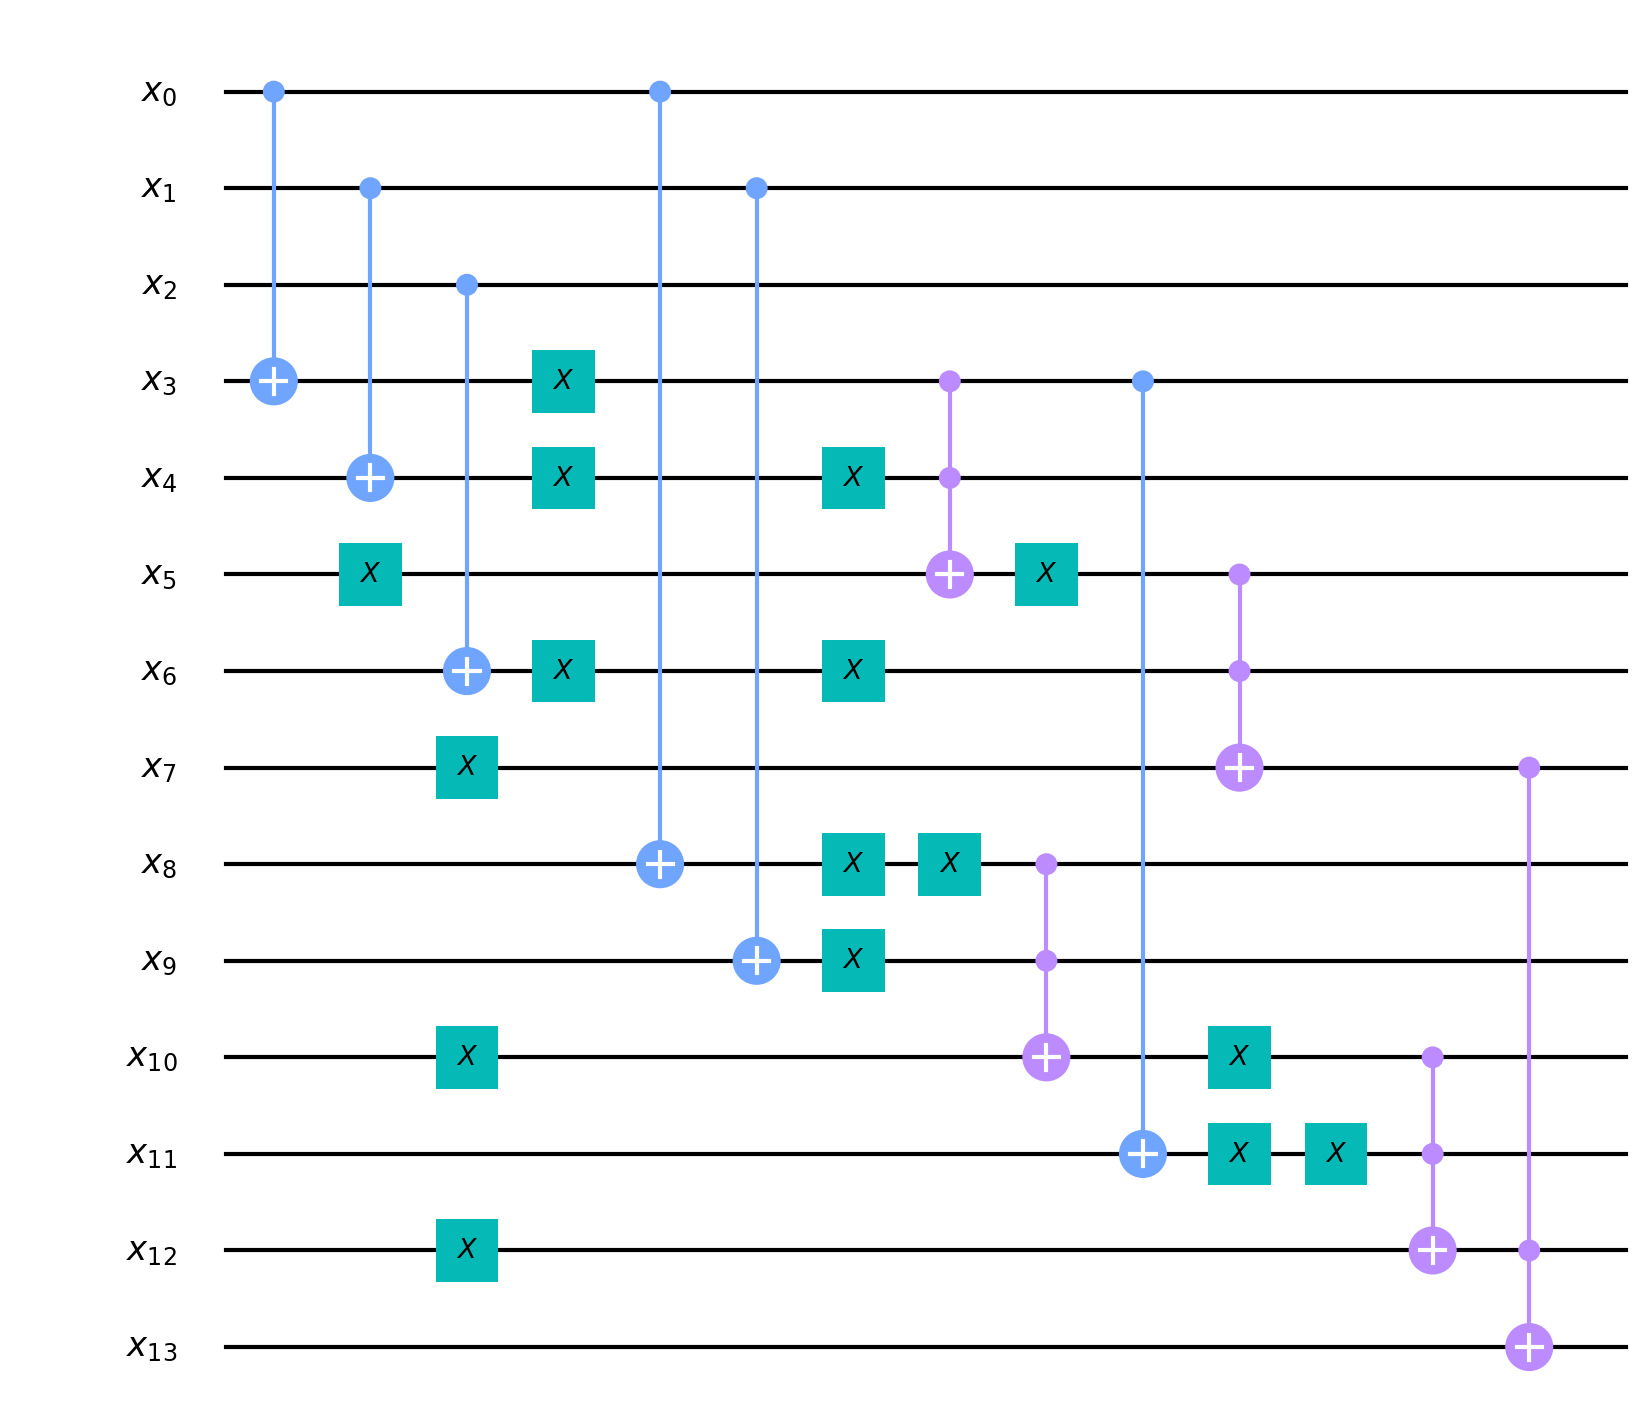
\includegraphics[scale=0.4]{example6.png}
				\caption{CNF circuit}
			\end{figure}
	
			To conclude with this section we still need to define the fundamental operation that allows us to retrieve the information from a qubit. As we have already said for qubits, while our algorithm is running, they posses the superposition property which makes them not to be at a certain instant in an exact place. To access the qubit information we want to understand if at that instance it is placed in either the 0 or the 1 position. The operation that allows to bring the information carried by a qubit to a result, thus something interpretable is called \emph{measurement}. Measurements will be implemented on the relevant qubits of our quantum computer so that we can see at the end of the algorithm which is the real quantum state in which we are arrived. By measuring a qubit we are asking which is the highest probability of the qubit for being 1 or 0. Measurement is represented with the following block in a quantum circuit:
			
			\begin{figure}[h]
				\centering
				\mbox{
					\Qcircuit @C=1em @R= 1em {
						& \meter & \qw 
				}}
				\caption{The measurement gate}
			\end{figure}
		
			It is important to understand that the outcome of a measurement will then be brought on a classical register where we will collect all the partial results measured from the relevant qubits of our circuit. As we saw in the introduction, the sad part of the story is that once we have measured a qubit it collapses to what we have called a "boring" unitary bit. This concept needs to be remembered also for what concerns the problem of copying a qubit that we will see later. Hence it is important to pose another conclusion to the list.
			
			\paragraph{Conclusion 3:} \emph{The state of the quantum system after a measurement collapses to a linear combination of only those basis states that are consistent with the outcome of the measurement. The original quantum state is no longer recoverable.}	
				
		\subsection{The Quantum Computer}
		\label{sec:quantumComputer}
			We now have all the necessary to define the quantum device, and thanks to this formalism we will also be able to define further important conclusions, obtained by putting together what we have seen so far. \\
			
			A quantum computer is not that different from how we consider a classical one in a general point of view. The device has a state and it evolves in other states by performing operations. The model of computation that is considered to formalize it is the quantum circuit model, which works as follows:
			
			\begin{itemize}
				\item The quantum computer has a \emph{state} that is stored in a quantum register, initialized in a certain way at the beginning of the computation
				
				\item \emph{Quantum operations} applied on a state allow the quantum computer to evolve from a state to another
				
				\item At the end of the computation the information stored in the quantum register, thus the final state, contains the result
			\end{itemize}
		
			Now it should be clear what to implement a quantum algorithm means and how the computation of a quantum algorithm is carried out on a quantum computer. Quantum algorithms are implemented on a quantum computer that provides a certain number of qubits to store the state. It is the programmer, knowing the quantum operations that we described in the previous section, who will make the states evolve in order to reach the one that contains the result. The best the quantum computer is realized the smaller the noise in the circuit will be. This means that the state will evolve with higher probability to the following expected one and that the measurements on the final state will return the correct result with a highest probability. \\
			
			To conclude with this part and start to study our first relevant quantum algorithm, we still have to clarify the two most important features related properly to quantum algorithms. We have seen that measuring a quantum state makes it collapse so that it can not be reused. Hence, it seems natural to look for a way to copy a quantum state, for example to continue with another computation. However, in particular because of the property of quantum gates to be unitary matrices it turns out that cloning a quantum state is not possible. This yields to another important conclusion that we have always to keep in mind while defining quantum algorithms.
			
			\paragraph{Conclusion 4:} \label{conc:noCloning} \emph{It is impossible to clone quantum states}.\\
			
			Whenever we run a circuit that produces an output quantum state, in general we can reproduce the output quantum state by only repeating all the steps of the algorithm.
			Another important aspect concerns the initialization of the quantum computer before starting to compute the algorithm. As we mentioned when we defined the Hadamard gate, by applying multiple Hadamards on the entire quantum state we set the state to a uniform superposition. It is here that we can feel another time the extreme power of quantum computing with respect to its classical counterpart.
			
			\paragraph{Conclusion 5:} \label{conc:superposition} \emph{Applying operations on a quantum device whose state is in a uniform superposition allows to apply them simultaneously to all possible binary strings thanks to linearity.} 
			
		\subsection{Grover's Algorithm}
		\label{sec:grover}
			Being now able to understand what a quantum algorithm is and how it can be implemented on a quantum circuit, we can start to consider one of the most important algorithms that is used in quantum computing. Thanks to Grover's algorithm we will be able to appreciate how a real quantum algorithm is implemented and why we actually obtain a speedup with respect to its classical counterpart. This algorithm, as it is described in the paper \cite[Lov K. Grover]{grover}, is a search algorithm in particular focused on looking for a certain element in a database. As we will precisely describe later, search algorithms are implemented with respect to a function $f$ which allows us to determine whether we found or not the element that we are looking for. The most important feature we will conclude is the \textbf{quadratic} speedup with respect to the most efficient search algorithm that we can implement classically. To exploit this enhancement we will use Grover's algorithm to solve the SAT problem and compare the complexity with a very efficient classical algorithm. 
			
			\paragraph{Basic Idea:} \emph{Start with the uniform superposition of all basis states, and iteratively increase the coefficients of basis states that correspond to binary strings for which an unknown function gives output 1.} \\
			
			This means that iteratively we will perform a set of operations that allow to increment the coefficient of the correct solution that will be retrieved in the final state thanks to the measurement operation. The algorithm requires $q = n + 1$ qubits to perform the basic operations but we will see in our implementation, as in many generalized cases happens, that some more qubits will be needed in order to perform intermediate steps that allow to generalize the algorithm. The qubits used to perform intermediate operations are typically called \emph{ancillary qubits} and it is very important to manage them as best as we can to prevent their exponential growth, caring of the \emph{no-cloning} conclusion we defined before.
			
			\paragraph{Outline:} \emph{Grover's algorithm starts with the uniform superposition of all basis states on n qubits. The last $n + 1$ qubit is already an auxiliary qubit and it is initialized as $H\ket{1}$. Thus we obtain the initial quantum state $\ket{\psi_0}$ and the following steps are iteratively repeated:}
			\begin{enumerate}
				\item Flip the sign of the vectors for which $U_f$ gives output 1.
				\item Invert all the coefficients of the quantum state around the average coefficient.
			\end{enumerate}
			A full cycle of these iterations increases the coefficients of the vectors that have been flipped at the first step. Continuing to iterate these steps allows to make the coefficient get always nearer to 1 for the correct solution until we perform the measurement. This phenomenon is known as \textbf{Amplitude Amplification} and it is the basis of Grover's algorithm. This quantum technique has an important possible drawback when used in Grover's search: \emph{the number of times that the steps have to repeated is not known a-priori, there are theoretical numbers that can be used, and by doing too less or too many iterations may result in finding a completely wrong solution!} \\
		
			Considering now the function we are interested in to implement Grover's algorithm we first consider how a classical search would allow to find a solution and then we define the 3 steps that are necessary to implement the quantum algorithm. Let $f:\{0,1\}^n \rightarrow \{0,1\}$, and assume that there exists a unique vector $\underline{s}\in\{0,1\}^n : f(\underline{s}) = 1$, i.e., there is a unique element in the domain of the function that yields output 1. We want to determine $\underline{s}$. The algorithm will run assuming that the function $f$ is encoded by a unitary matrix that we will consider as $U_f$.
			
			\subsubsection{Classical Grover}
			\label{sec:groverClass}
				Now that we know how the search problem is defined, given the function $f$ introduced above, we have clear in mind that classical search cannot do better than $\mathcal{O}(2^n)$ operations. Indeed, as we will precisely describe at the beginning of the SAT implementation section (\ref{sec:satImpl}), we can design classical algorithms in both deterministic or nondeterministic paradigms. Nondeterminism is obtained with randomization and it provides in general more efficient algorithms but very complex to be designed and debugged. Any deterministic classical algorithm may need to explore all $2^n$ possible input values before finding $\underline{s}$: given any deterministic classical algorithm, there exists a permutation $\pi$ of $\{0,1\}^n$ that represents the longest execution path of such algorithm. Then, if $\underline{s} = \pi(\underline{1})$ the algorithm will require $2^n$ \textbf{queries} (important to understand query complexity described at \ref{conc:queryCompl}) to determine the answer, which is clearly the worst case. At the same time, a randomized algorithm requires $\mathcal{O}(2^n)$ function calls to have at least a constant positive probability to determine $\underline{s}$; the expected number of function calls to determine the answer is approximately $2^{n-1}$.
			
			\subsubsection{Quantum Grover}
			\label{sec:groverQuant}
				In the beginning of the section we have provided all the elements that we need to realize Grover's algorithm, as we said there are 3 steps that are iteratively repeated in order to obtain the best solution possible. We now want to give some more details about these steps:
				
				\begin{enumerate}
					\item \textbf{Initialization:}
					The algorithm is initialized by applying the operation $\bigotimes^{n+1}\mathcal{H}(\bigotimes^n I\otimes X)$ onto the state $|\underline{0}\rangle_{n+1}$. This brings the basis state in uniform superposition and the initial coefficients of the state $\ket{\psi}$ are real numbers. 
					
					\item \textbf{Sign Flip:}
					To flip the sign of the target state $\ket{\underline{s}}_n \otimes \frac{1}{\sqrt{2}}(\ket{0}-\ket{1})$, we apply $U_f$ to $\ket{\psi}$. In fact we can always think of the n + 1 qubit as being in the state $\frac{1}{\sqrt{2}}(\ket{0}-\ket{1})$ and \emph{unentangled} from the rest of the qubits, with the sign flip afflicting only the first n qubits. Therefore, the state we obtain by applying $\mathcal{U}_f$ to $\ket{\psi}$ is the same as $\ket{\psi}$ except that the sign of $\ket{\underline{s}}_n \otimes \frac{1}{\sqrt{2}}(\ket{0}-\ket{1})$ has been flipped.
					
					\item \textbf{Inversion about the average:}
					The last step consists of the inversion about the average of the state in order to modify the coefficients corresponding to the correct solution. This is a unitary operation that can be expressed by the following matrix:
					\begin{equation*}
						\centering
						W =
						\begin{pmatrix}
						\frac{2}{2^n}-1 & \frac{2}{2^n} & \cdots & \frac{2}{2^n} \vspace{3pt} \\
						\frac{2}{2^n} & \frac{2}{2^n}-1 & \cdots & \frac{2}{2^n} \\
						\vdots & \vdots & \ddots & \vdots \\
						\frac{2}{2^n} & \frac{2}{2^n} & \cdots & \frac{2}{2^n}-1
						\end{pmatrix}
						=
						\begin{pmatrix}
						\frac{2}{2^n} & \frac{2}{2^n} & \cdots & \frac{2}{2^n} \vspace{3pt} \\
						\frac{2}{2^n} & \frac{2}{2^n} & \cdots & \frac{2}{2^n} \\
						\vdots & \vdots & \ddots & \vdots \\
						\frac{2}{2^n} & \frac{2}{2^n} & \cdots & \frac{2}{2^n}
						\end{pmatrix}
						- \otimes^{n}I
					\end{equation*}
					where the denominator $\frac{1}{2^n}$ computes the average coefficient, the numerator 2 of the fraction takes twice the average, and finally we subtract the identity to subtract each individual coefficient from twice the average. Thanks to the definition of the Hadamard gate we can show that W can be written as:
					\begin{equation*}
					\centering
					W = (-\otimes^n\mathcal{H})D(\otimes^n\mathcal{H})
					\end{equation*}
					where D is a diagonal matrix $diag(-1,1,\cdots,1)$ of size $2^n$. This expression trivially shows that $W$ is unitary in fact $\bigotimes^n\mathcal{H}$ is unitary and D is diagonal with ones on its diagonal. Thus we can summarize the analysis of the inversion of the average by concluding that it can be performed by applying $W = (-\bigotimes^n\mathcal{H})D(\bigotimes^n\mathcal{H})$ to the n qubits of interest.
				\end{enumerate} 

	\section{Computational Theory}
	\label{sec:computationalTheory}
		It is important to give a brief introduction also about computational theory, in particular to understand how we are able to compare the execution of a classical with a quantum algorithm but also to grasp why the SAT has been chosen as the reference algorithm to carry on the entire paper. In this section we want to address quickly the basic computational definitions we need to evaluate the complexity of a classical algorithm and understand how these definitions are applied in quantum algorithms. We will see that the quadratic speedup we achieved thanks to Grover's algorithm provides enhancements in a slight different computation complexity definition with respect to the one we are used to consider. \\
		
		In the classical computational theory we are interested in determining two major types of issues:
		
		\begin{enumerate}
			\item Evaluate the \emph{complexity} of a given algorithm $A$ to solve a problem $P$
			
			\item Evaluate the \emph{inherent difficulty} of a given problem $P$
		\end{enumerate}
	
		\subsection{Algorithm Complexity}
		\label{sec:algorithmComplexity}
			As we have studied, being computer scientist engineers, one of the most important things to solve a problem is to choose the best algorithm in terms of performances to solve each of the possible instances of the problem. But how do we evaluate the performances of an algorithm?
			
			\paragraph{Definition (Computing Time):} \emph{The computing time of an algorithm is evaluated in terms of elementary operations needed to solve a given instance $I$. In this definition we assume that all elementary operations require one unit of time.} \\
			
			It is clear that the number of elementary operations depends on the size of the instance $I$. The biggest the instance it is, the highest the computing time will be. The \textbf{size} of an instance can be considered as the number of bits needed to encode that specific instance. There are two types of complexity that influence the choice of an algorithm:
			
			\begin{itemize}
				\item \textbf{Time Complexity:} we want to identify a function $f(n)$ such that, for every instance $I$ of size at most n the number of elementary operations to solve the instance is smaller or equal to $f(n)$.
				
				\item \textbf{Space Complexity:} we want to identify a function $g(n)$ such that, for every instance $I$ of size n the number of bits needed to encode it is smaller or equal to $g(n)$.
			\end{itemize}
			
			In the comparison between the classical and the quantum solver for the SAT we will mainly focus on time complexity where we can prove the quadratic speedup thanks to Grover's search algorithm. However we do not have to neglect space complexity: we have said that it is an issue for the encoding of a quantum state with respect to the classical approach and the no-cloning principle will make us consider techniques to reuse qubits in order to reduce the exponential growth that we have described. \\
			
			As we know, the function $f(n)$ is expressed in asymptotic terms using the \emph{big-O notation}, and thanks to it we are able to make a very important distinction in classical algorithms.
			
			\paragraph{Definition (Polynomial Algorithm):} \emph{an algorithm is polynomial if it requires, in the worst case, a number of elementary operations $f(n)=\mathcal{O}(n^k)$ where n is the size of the instance and k a constant.}
			
			\paragraph{Definition (Exponential Algorithm):} \emph{an algorithm is exponential if it requires, in the worst case, a number of elementary operations $f(n)=\mathcal{O}(2^n)$ where n is the size of the instance.} \\
			
			We always look for polynomial algorithms to solve our problems but for some interesting case we haven't still found a better solution than an exponential algorithm. As we will see in section \ref{sec:satClassical} very efficient algorithms have been studied to reduce the complexity of the solver for the SAT problem but the best we can achieve is to decrease the base of the exponential until $\mathcal{O}(1.30704^n)$ (randomized classical algorithm). This is already an extreme enhancement, decreasing the base almost to 1, which would lead the algorithm to be constant time. Imagine now that Grover search is able to quadratically speedup this complexity and grasp once more the advantages of quantum algorithms.
		
		\subsection{Inherent Difficulty}
		\label{sec:inherentDifficulty}
			In this section we are going to formalize the theory that studies which of the algorithms is the best to solve a specific problem. Intuitively we are looking for the complexity of the most efficient algorithm that could ever be designed for that problem.
			
			\paragraph{Definition (Simple Problem):} \emph{an algorithm $P$ is polynomially solvable ("easy"), if there is a polynomial-time algorithm providing an optimal solution for every of its instances.} \\
			
			Thus which are difficult problem? Actually we will give a more precise definition by using the $hard$ word, in fact it does not suffice to have an algorithm that solves a problem in exponential time to say that it is difficult. It may be that we have not still found the algorithm able to solve it in polynomial time! There are several problems that seem to be "difficult", for example: \emph{the Travelling Salesman Problem, the SAT, graphs colouring...}
		
		\subsection{NP-completeness Theory}
		\label{sec:npCompleteness}
			To continue the study of algorithms we want to reach the definitions of the complexity classes $P$ and $NP$. With this classification we will finally be able to understand why we decided to choose the SAT as the reference problem for this paper. To simplify the discussion we will consider the \emph{recognition version} of a problem without loosing any kind of generality.
			
			\paragraph{Definition (Recognition Version):} \emph{a recognition problem is a problem whose solution is either "yes" or "no".} \\
			
			To every optimization problem we can associate its recognition version, always considering the following assumption: any optimization problem is at least as difficult as its recognition version. This shows why concluding that a recognition problem is "difficult" implies that its original version is "difficult" too. Now that we know the definition of recognition problems we can provide the first very important definition of the complexity class in which we hope to find the algorithm that solves our problem.
			
			\paragraph{Definition (Complexity P-class):} \emph{$\mathcal{P}$ denotes the class of all recognition problems that can be solved in polynomial time}. \\
			
			An important conclusion shows that $\mathcal{P}$ can be formally defined in terms of deterministic Turing machines. This is very interesting for us, in particular recalling what we concluded at \ref{conc:qcTuring}. The other complexity class we do not hope to retrieve our algorithm in,  is a superclass of the one we have just presented and it is defined as follows.
			
			\paragraph{Definition (Complexity NP-class):} \emph{$\mathcal{N}\mathcal{P}$ denotes the class of all recognition problems such that, for each instance with “yes” answer, there exists a concise proof which allows to verify in polynomial time that the answer is “yes”.} \\
		
			A trivial example is the 3-SAT recognition problem: given a clause we are able in polynomial time to establish whether the problem is satisfiable or not. From the definitions we have just provided it is clear that the $\mathcal{N}\mathcal{P}$ includes the $\mathcal{P}$, but nothing more can be said among these two classes. It is in fact one of the \emph{millennial problems} the one to establish whether $\mathcal{N}\mathcal{P}$ coincides with $\mathcal{P}$ or that the inclusion is strict. \\
			
			To understand the decision of choosing the SAT as the reference algorithm we still need some definitions. In particular we will see that thanks to the SAT we are able to classify several algorithms in the classes we have just presented. In order to do so we need a criterion that allows to classify an algorithm thanks to its intrinsic difficulty, identifying the most difficult ones in $\mathcal{N}\mathcal{P}$.
			
			\paragraph{Definition (Polynomial Time Reduction):} \emph{Let $\mathcal{P}_1, \mathcal{P}_2 \in \mathcal{N}\mathcal{P}$, then $\mathcal{P}_1$ reduces in polynomial time to $\mathcal{P}_2$ ($\mathcal{P}_1 \propto \mathcal{P}_2$) if there exists an algorithm to solve $\mathcal{P}_1$ which:}
			\begin{enumerate}[label=(\roman*)]
				\item \emph{uses (once or several times) a hypothetical algorithm for $\mathcal{P}_2$ as a subroutine}
				
				\item \emph{the algorithm for $\mathcal{P}_1$ runs in polynomial time if we assume that the algorithm for $\mathcal{P}_2$ runs in constant time}
			\end{enumerate}
		
			Thanks to this first definition we can draw a first conclusion that allows us to classify an algorithm in the $\mathcal{P}$ class: \emph{if $\mathcal{P}_1\propto\mathcal{P}_2$ and $\mathcal{P}_2$ admits a polynomial-time algorithm, then also $\mathcal{P}_1$ can be solved in polynomial time. In formulas:}
			
			\begin{equation*}
				\centering
				(\mathcal{P}_1\propto\mathcal{P}_2) \land (\mathcal{P}_2 \in \mathcal{P}) \implies \mathcal{P}_1 \in \mathcal{P}
			\end{equation*}
		
			Now that we know how to classify polynomial time algorithms we need a similar criterion also for the problems that belong to the $\mathcal{N}\mathcal{P}$ class. The discussion is now more delicate, in particular we need another definition in order to identify a very special subclass containing the most relevant difficult problems contained in $\mathcal{N}\mathcal{P}$.
			
			\paragraph{Definition ($\mathcal{N}\mathcal{P}$-complete Problems):} \emph{a problem $P$ is $\mathcal{N}\mathcal{P}$-complete if and only if:}
			\begin{enumerate}[label=(\roman*)]
				\item $P$ belongs to $\mathcal{N}\mathcal{P}$
				
				\item every other problem $P^{'}\in\mathcal{N}\mathcal{P}$ can be reduced to $P$ in polynomial time ($P^{'}\propto P$)
			\end{enumerate}
			 
			 This definition has a very important consequence related to the millennial problem we defined before. If there existed any polynomial-time algorithm for any $\mathcal{N}\mathcal{P}$-complete problem, then all problems in $\mathcal{N}\mathcal{P}$ can be solved in polynomial time. Thus we would have demonstrated that: $\mathcal{P}=\mathcal{N}\mathcal{P}$. Many studies show that the equality is very unlikely, thus it is conceived that the relation between the two classes is a strict inclusion. However, this allows us to say that $\mathcal{N}\mathcal{P}$-completeness provides a strong evidence that a problem is \emph{inherently difficult}. Now, to show that $P_2\in\mathcal{N}\mathcal{P}$ is $\mathcal{N}\mathcal{P}$-complete it suffices to show that an $\mathcal{N}\mathcal{P}$-complete problem $P_1$ reduces in polynomial time to $P_2$. More formally:
			 \begin{equation*}
			 	\centering
			 	P\propto P_1, \forall P\in\mathcal{N}\mathcal{P} \land P_1 \propto P_2 \overset{transitivity}{\implies} P\propto P_2, \forall P\in \mathcal{N}\mathcal{P}
			 \end{equation*}
			 
			 But does there exist an $\mathcal{N}\mathcal{P}$-complete algorithm that allows us to exploit this implication? The answer was provided by Stephen Arthur Cook in 1971 when he proved that the SAT is $\mathcal{N}\mathcal{P}$-complete (\cite[Stephen A. Cook]{CookSAT}). This conclusion has brought enormous advantages to the complexity theory, an example are the 21 discrete optimization problems shown to be $\mathcal{N}\mathcal{P}$-complete by Richard Karp in 1974. To conclude this section thanks to the definition of $\mathcal{N}\mathcal{P}$-complete problems we can give a further classification.
			 
			 \paragraph{Definition ($\mathcal{N}\mathcal{P}$-Hard Problem):} \emph{a problem is $\mathcal{N}\mathcal{P}$-Hard if every problem in $\mathcal{N}\mathcal{P}$ can be reduced to it in polynomial time (even if it does not belong to $\mathcal{N}\mathcal{P}$).} \\
			 
			 This last definition allows us to formulate a very important observation that relates ones more a problem with its recognition version: all optimization problems with an $\mathcal{N}\mathcal{P}$-complete recognition version are $\mathcal{N}\mathcal{P}$-Hard.
			 
			 It should be now clear why we decided to choose the SAT as the example for drive the entire comparison between how the classical solver performs with respect to its quantum counterpart. The conceptual part of this paper is now arrived to its epilogue and we can start the real comparison. The next two subsections are used to introduce first the formal definition of the SAT problem and then to understand how quantum algorithms impact onto the $\mathcal{N}\mathcal{P}$ class.
		
		\subsection{SAT Problem}
		\label{sec:sat}
			Let $X\equiv\{x_1, x_2, \cdots, x_n\}$ be a set. Then $x_k$ and its negations $\overline{x}_k\;(k=1, 2, \cdots, n)$ are called literals and the set of all such literals is denoted by $X^{'}=\{x_1,\overline{x}_1,\cdots, x_n, \overline{x}_n\}$. The set of all subsets of $X^{'}$ is denoted by $\mathcal{F}(X^{'})$ and an element $C\in\mathcal{F}(X^{'})$ is called a clause. We consider a truth assignment to all variables $x_k$. If we can assign the truth value to at least one element of $C$, then $C$ is called satisfiable. When $C$ is satisfiable, the truth value $t(C)$ of $C$ is regarded as true, otherwise, that of $C$ is false. Take the truth values as true "1" while false "0". Then 
			\begin{equation*}
				\centering
				C\;is\;satisfiable\iff t(C)=1
			\end{equation*}
			Let $L=\{0,1\}$ be a Boolean lattice with usual join $\lor$ and meet $\land$, and $t(x)$ be the truth value of a literal $x$ in $X$. Then the truth value of a clause $C$ is written as
			\begin{equation*}
				\centering
				t(C) = \lor_{x\in C}t(x) 
			\end{equation*}
			Further  a set $\mathcal{C}$ of all clauses $C_j\;(j = 1, 2, \cdots, m)$ is called \emph{satisfiable} if and only if the meet of all truth values of $C_j$ is 1:
			\begin{equation*}
				\centering
				t(\mathcal{C}) = \land_{j = 1}^{m}t(C_j) = 1 
			\end{equation*}
			
			Finally the formal definition of the most general formulation of the SAT problem is written as follows.
			
			\paragraph{Definition (SAT Problem):} \emph{given a set $X\equiv \{x_1,x_2,\cdots,x_n\}$ and a set $\mathcal{C}={C_1,C_2,\cdots,C_m}$ of clauses, determine whether $\mathcal{C}$ is satisfiable or not.} \\
			
			Hence it is the problem to determine whether it exists a truth assignment to make $\mathcal{C}$ satisfiable. As we have already mentioned the satisfiability problem can be also described as the problem of asking if there exists an assignment to the literals of its clauses that makes the \emph{Conjunctive Normal Form} to have value 1. The CNF also called \emph{Product of Sums} (POS) is obtained by the conjunction of the clauses written as the disjunction of their literals. \\
			
			Now that we know the formal definition of the SAT it is important to understand some of its specific formulations, in particular the ones that we considered during this study and that I decided to implement for the comparison. As it is reported in almost every paper, the SAT is in fact denoted as k-SAT. The k indicates the maximum number of variables that each clause can be composed of; if we look at the example \ref{ex:c6} we have a 3-SAT problem with $n = 3$ variables and $m=2$ clauses both of length 3. Thus we can have in general a 3-SAT problem defined over n variables and m clauses. The precise definition of the implementations of the SAT that we considered are presented in the last section (\ref{sec:satImpl}), here it is the list of all its formulations and some important features of each in particular with respect their complexity:
			
			\begin{itemize}
				\item At first it is important to understand that the exponential growth of the instance in modern solvers for an SAT instance is caused by the maximal length of each clause. Thus the highest the k will be the more time will be required by our solver to solve the problem. The number of clauses instead do not influence the time complexity while we will need more space to encode every additional clause; but let's focus always on time complexity
				
				\item The recognition version of every k-SAT instance can be solved in polynomial time. Thus we are able to design an algorithm that is able to answer "yes" when a given clause makes the formulation satisfiable or "no" otherwise, in polynomial time.
				
				\item It has been proved that the general versions of the 1-SAT and the 2-SAT versions can be solved in polynomial time. The solvers we implemented are generalized to the case of k clauses as we could compare also the polynomial time solutions; we will see that while in this case the enhancement provided by the quantum version is not that significant we perceive problems for the exponential growth of the size of the instance of the quantum device!
				
				\item The 3-SAT version is the simplest and significant case from which we can start the comparison. As we can see in the literature it is the most studied case and all the efficient solvers that have been implemented consider it as reference. It would be in fact sufficient to find an algorithm that solves it in polynomial time and generalize it for its further formulations.
				
				\item The most general quantum solver of an SAT formulation combines classical efficient algorithms with Grover's search and qiskit version is already the best. We considered it to make the general comparison between k-SAT problems while we studied a simplified version to see in action the specific quantum steps of Grover's algorithm.
				
				\item The exactly-1-3-SAT problem is formalized as follows: \\
				
				\hspace{0.3cm} \textbf{INPUT:} SAT formula in conjunctive normal form $\land_{j = 1}^{m}C_j$ over n Boolean variables $x_1,x_2,\cdots,x_n$ with 3 literals per clause $C_1,C_2,\cdots,C_m$ \\
				
				\hspace{0.3cm} \textbf{OUTPUT:} Does there exist an assignment $x_1,x_2,\cdots,x_n$ such that every clause $C_1,C_2,\cdots,C_m$ has \textbf{exactly one} \emph{true} literal?
				
				The exactly-1-3-SAT has been proved to be still a $\mathcal{N}\mathcal{P}$-Hard problem.
			\end{itemize}
			
		\subsection{Can we solve NP-hard problems?}
		\label{sec:npHardProblems}
			In \cite[G.Nannicini, 2020]{introNoPh} is highlighted an important remark that we have now to consider, finally competing with both the quantum computing world and the computational complexity theory. The answer to this section can be included in the important conclusions we are highlighting in this paper, in fact we can formulate it as follows.
			
			\paragraph{Conclusion 6:} \emph{even if we can easily create a uniform superposition of all basis states, the rules of measurement imply that using just this easily-obtained superposition does not allow us satisfactorily solve $\mathcal{N}\mathcal{P}$-complete problems, such as, for example, SAT.} \\
			
			As we explained in Grover's algorithm to solve the SAT problem (section \ref{sec:grover}), considering a circuit of $q = n + 1$ qubits and performing the measurement of this state will return a binary string that satisfies the SAT formula if and only if the last qubit has value 1 after the measurement. This happens with a probability that depends on the number of binary assignments that satisfy the formula. If the SAT problem at hand is solved by exactly $\epsilon$ assignments out of $2^n$ possible assignments, then the probability of finding the solution after one measurement is $\frac{\epsilon}{2^n}$: we have just randomly sampled a binary string hoping that it satisfies the SAT formula. Clearly, this is not a good algorithm. Thanks to what we have just pointed out we can draw another important conclusion to be considered with respect to the complexity classes that we identified.
			
			\paragraph{Conclusion 7:} \emph{in general solving $\mathcal{N}\mathcal{P}$-Hard problems in polynomial time with quantum computers is not believed to be possible.} \\
			
			The literature shows that the BQP class, the class of problems solvable in polynomial time by a quantum computer with bounded error probability, does not contain the class $\mathcal{N}\mathcal{P}$. Of course the proof is not available yet, because showing that $\mathcal{N}\mathcal{P}\nsubseteq BQP$ would resolve the millennial problem \textbf{P vs NP}. Even if we cannot solve all "difficult" problems in polynomial time using a quantum computer, we will see with the implementation of our SAT solver a significant speedup from every other classical implementation. The basic principle on which our quantum algorithm works is to start with the uniform superposition of the state representing the clauses and perform three steps that allow to modify the coefficients of the correct solution so that in the end, when we will measure the final state, it will result the most probable.
		
	\section{SAT Implementation}
	\label{sec:satImpl}
		We have finally reached the heart of this paper. Having now all the necessary fundamental concepts of quantum computing and of the problem we want to study, it is possible to put everything together and make the comparison we have been talking until now. To understand how to compare a classical algorithm with its respective quantum counterpart we will need one last definition and some further considerations on the complexities that are now achieved by the most efficient classical algorithms for the problem of solving the SAT. The section starts with the formal definition of four problems that we decided to use for giving a precise description of how the algorithms behave while solving the problems they describe. Then we continue with the classical implementation (\ref{sec:satClassical}) to describe the complexities by showing in the end the characteristics of the algorithm we decided to use in order to realize the comparison. Then in the quantum part (\ref{sec:satQuantum}), in the same way we describe how the complexities are enhanced thanks to the implementations we realized and which are the results we obtained with respect to the four SAT instances we decided to use. In the end, thanks to all the information obtained from the two implementations we will draw the comparison. \\
	
		As we mentioned, before going deep inside the implementation of the algorithms we need to define a concept that may result confusing for what we have said until now about computational complexity. However, we needed what studied in section \ref{sec:computationalTheory} to identify the main issues of complexity in both a classical and quantum world. To conclude our work and realize a comparison between the SAT solvers we need to consider another type of complexity in particular related to all those algorithms that belong to the family of \textbf{quantum searching algorithms}. As we already said, thanks to Grover we are able to perform a search of our solution to the SAT problem by exploiting quantum physics features and to compare the quadratic speedup obtained we need to consider the following very important conclusion.
		
		\paragraph{Conclusion 8:} \label{conc:queryCompl} \emph{The complexity of a quantum algorithm that belongs to the search class is determined only in terms of the number of the calls to the function f. This model is known as query complexity, because it defines the complexity of an algorithm as the number of queries to a given function (in this case, f). Query complexity is used as a model to answer important theoretical questions. There are many quantum algorithms that yield speedups under the query complexity model, but some others, e.g., Shor's algorithm, are faster than (known) classical algorithms under the more traditional computational complexity model, i.e., number of basic operations.}
	
		\subsection{SAT Instances}
		\label{sec:satInstances}
			In order to compare the execution of the classical and the quantum solvers we decide to report here the four most relevant cases we used during our study. First of all we will consider three cases of 3-SAT problems followed by a 4-SAT one in order to show the results for more than 3 clauses and with a size greater than 3. In all the formulation, considering the problem of the exponential growth of the qubits in the case of considering more variables we focused on the case where the length k of the clauses coincides with the number n of variables of the problem. In this way we do not loose generalization and we do not waste space to consider more than the necessary variables. The following subsections contain the formal definition of the problems we can find in the repository in the folder \textsc{.../Input} for each implementation. From now on we will call the three instances as \textbf{Problem 1 - Problem 2 - Problem 3 - Problem 4}.
			
			\subsubsection{Problem 1 (3-SAT Instance)}
			\label{sec:problem1}
				Consider the 3-SAT problem defined over the set of variables $X=\{x_1, x_2, x_3\}$ and the three clauses $C=\{C_1, C_2, C_3\}$, such that:
				\begin{center}
					$C_1 = \{x_1, x_2, \neg x_3\}$ \\
					$C_2 = \{\neg x_1, \neg x_2, \neg x_3\}$ \\
					$C_3 = \{\neg x_1, x_2, x_3\}$
				\end{center}
				That corresponds to the following conjunctive normal form:
				\begin{equation*}
					\centering
					CNF \equiv (x_1 \lor x_2 \lor \neg x_3) 
							\land (\neg x_1 \lor \neg x_2 \lor \neg x_3)
							\land (\neg x_1 \lor x_2 \lor x_3)
				\end{equation*}
				
			\subsubsection{Problem 2 (3-SAT Instance)}
			\label{sec:problem2}
			Consider the 3-SAT problem defined over the set of variables $X=\{x_1, x_2, x_3, x_4, x_5\}$ and the five clauses $C=\{C_1, C_2, C_3, C_4, C_5\}$, such that:
			\begin{center}
				$C_1 = \{x_1, \neg x_2, \neg x_3\}$ \\
				$C_2 = \{x_2, \neg x_3, \neg x_4\}$ \\
				$C_3 = \{x_3, \neg x_4, \neg x_5\}$ \\
				$C_4 = \{x_4, \neg x_5, \neg x_1\}$ \\
				$C_5 = \{x_5, \neg x_3, \neg x_4\}$
			\end{center}
			That corresponds to the following conjunctive normal form:
			\begin{equation*}
				\centering
				CNF \equiv (x_1 \lor \neg x_2 \lor \neg x_3)
						\land (x_2 \lor \neg x_3 \lor \neg x_4)
						\land (x_3 \lor \neg x_4 \lor \neg x_5)
						\land (x_4 \lor \neg x_5 \lor \neg x_1)
						\land (x_5 \lor \neg x_3 \lor \neg x_4)
			\end{equation*}
			
			\subsubsection{Problem 3 (3-SAT Instance)}
			\label{sec:problem3}
				Consider the 3-SAT problem defined over the set of variables $X=\{x_1, x_2, x_3\}$ and the three clauses $C=\{C_1, C_2, C_3\}$, such that:
				\begin{center}
					$C_1 = \{x_1, x_2, \neg x_3\}$ \\
					$C_2 = \{\neg x_1, x_2, \neg x_3\}$ \\
					$C_3 = \{x_1, x_2, x_3\}$
				\end{center}
				That corresponds to the following conjunctive normal form:
				\begin{equation*}
				\centering
				CNF \equiv (x_1 \lor x_2 \lor \neg x_3) 
				\land (\neg x_1 \lor x_2 \lor \neg x_3)
				\land (x_1 \lor x_2 \lor x_3)
				\end{equation*}
			
			\subsubsection{Problem 4 (4-SAT Instance)}
			\label{sec:problem4}
				Consider the 4-SAT problem defined over the set of variables $X=\{x_1, x_2, x_3, x_4\}$ and the four clauses $C=\{C_1, C_2, C_3, C_4\}$, such that:
				\begin{center}
					$C_1 = \{x_1, \neg x_2, \neg x_3, \neg x_4\}$\\
					$C_2 = \{\neg x_1, x_2, \neg x_4\}$\\
					$C_3 = \{\neg x_1, \neg x_2, \neg x_3, x_4\}$\\
					$C_4 = \{\neg x_2, x_3, \neg x_4\}$
				\end{center}
				That corresponds to the following conjunctive normal form:
				\begin{equation*}
					\centering
					CNF \equiv (x_1 \lor \neg x_2 \lor \neg x_3 \lor \neg x_4)
							\land (\neg x_1 \lor x_2 \lor \neg x_4)
							\land (\neg x_1 \lor \neg x_2 \lor \neg x_3 \lor x_4)
							\land (\neg x_2 \lor x_3 \lor \neg x_4)
				\end{equation*}
		
		\subsection{Classical}
		\label{sec:satClassical}
			The SAT problem, thanks to the importance it provided to the field of computational complexity when Cooks demonstrated its belonging to the $\mathcal{N}\mathcal{P}$-complete class, became the subject of several research studies. The researches followed all the same objective, that is the one of obtaining a polynomial solver for any instance of the SAT problem in order to prove the millennial problem of P vs NP. However nowadays we are not still able to find such an algorithm and thus a solution to the famous problem. \\
			
			Every year it is held a competition where the most competent computer scientists in the world compete in order to implement the best SAT solver in terms of computational complexity. Thanks to this event and to the huge research behind this problem, starting from deterministic algorithms forward to nondeterministic ones surprising results were obtained. The exciting part of these exponential time algorithms is their ability to reduce always more the basis of the general starting point of every search algorithm: $2^n$. As we see in the following list for the 3-SAT problem of deterministic and nondeterministic algorithms different approaches allow to reduce the 2 until the best result reached so far of: $\mathcal{O}(1.30704^n)$.
			
			\begin{itemize}
				\item	\cite[Kutzkov K., Scheder D.]{KutzkovScheder} $\mathcal{O}(1.439^n)$ \textbf{[Deterministic]}
				
				\item	\cite[Makino K., Tamaki S., Yamamoto M]{MakinoTamakiYamamoto} $\mathcal{O}(1.3303^n)$ \textbf{[Derandomized]}
				
				\item	\cite[Iwama K., Seto K., Takai T., Tamaki S.]{IwamaSetoTakai} $\mathcal{O}(1.32113^n)$ \textbf{[Randomized]}
				
				\item	\cite[Hertli T., Moser R. A., Scheder D.]{HertliMoserScheder} $\mathcal{O}(1.32065^n)$ \textbf{[Randomized]}
				
				\item	\cite[Hertli T.]{Hertli} $\mathcal{O}(1.30704^n)$ \textbf{[Randomized]}
			\end{itemize}
			
			\subsubsection{Solver}
			\label{sec:classicalSolver}
				We can now introduce the version of the solver considered to make the comparison between the classical and the quantum implementations. The aim was to find the best solver for the comparison, but in order to realize one as efficient as the those listed above would have required mathematical skills not relevant for our study. Hence I decided to start with a solver that is based on \emph{Knuth} SAT0 (\url{https://www-cs-faculty.stanford.edu/~knuth/programs/sat0.w}) solution in order to have a first comparison to test some particular instances of the k-SAT problem (with k ranging from 2 to 4). The solver implementation is available at \url{https://github.com/sahands/simple-sat}, even if based on the first of Knuth's SAT-solvers series it exploits some particular features that allow to handle in the best way the algorithm resolution over a general k-SAT formulation. \\
				
				The algorithm is a watch-list based backtracking algorithm based on the following features that allow to obtain an efficient version in terms of both time and space complexities:
				
				\begin{enumerate}[label=(\roman*)]
					\item To encode the formulation of a general k-SAT instance we need to represent it with the meaning of a CNF. Thus a set of clauses each containing variables, negated or not, in conjunction. To do so we may think to realize a list of all the clauses, but this does not help when in the algorithm we want to look for the variables in order to find a satisfying formula. Instead, unique number is assigned to each variable once it is encountered, starting from 0 and counting up, using a dictionary to keep track of the mapping. Then the positive variables encoded as number $x$ will be stored at position $2x$ and the negated one will be present at $2x+1$.
					
					\item It is a backtracking algorithm in which we try to assign true or false values to all variables, starting from the one at position 0 up to the last $n - 1$ one. The entire search space is of size $2^n$ but by pruning, only the best branches of the search tree will be explored.
					
					\item Watch-lists allow to manage easily the backtracking mechanism. For each clause to be satisfied we need in fact one literal to be true. As such, we can make each clause watch one of its literals, and ensure that the following \textbf{invariant} is maintained throughout the algorithm: \emph{all watched literals are either not assigned yet, or they have been assigned true}. Then we proceed assigning true or false values to variables, starting from 0 up to $n-1$. If we successfully assign true or false to every variable while maintaining the above variant, then we have an assignment that satisfies every clause.
					
					\item Every time we assign a value to a variable we have to ensure that the watch-list is updated accordingly. To do so efficiently, we need to keep a list of clauses that are currently watching a given literal. This is done thanks a double-ended queue which provides the best performances.
					
					\item During a backtracking step, assignments only go from 0 or 1 to None, the watch-list does not need to be updated at all to maintain the invariant. This is why the watch-list is the best approach and it means that the backtracking step will simply be changing the assignment of a variable back to None.
					
					\item Both recursive and iterative versions are present, we used the iterative one for out tests mainly for what Knuth says about his dislike to recursion. The SAT0 is in fact implemented in an iterative way.
				\end{enumerate}
			
			\subsubsection{Significant Results}
			\label{sec:classicResults}
				The classical solver runs efficiently the execution of the algorithm able to find the solutions of each of the problems provided. We see that each of the formulations are satisfiable and we notice that for how the encoding of each clause is managed none of the run instances provides the same result as the ones obtained in the exactly-1 formulation (\ref{sec:quantumResults}). Talking about complexity we used a very efficient deterministic algorithm based on the backtracking of the search tree, also managing the clauses in a way that does not bring to a repetition of the information needed. Hence in the comparison we can use the complexities of the methods cited above in order to consider also the case of nondeterministic algorithms.
				
		\subsection{Quantum}
		\label{sec:satQuantum}
			In this section we finally provide the description of the solvers we considered to realize the comparison. In order to face the implementation of a solver for the SAT problem we go through three different approaches that allow to understand how the final algorithm has been implemented. First with a jupyter notebook it is possible to understand the comparison from the most general formulation of the problem, thus a k-SAT instance. In the notebook we used qiskit's implementations to solve a big instance of the problem in order to see how it performed in a very complicate example. The decision version implementation instead is used to make some practice, in particular for the problem of realizing manually multiple qubit gates that the library does not support. In the end the exactly-1 k-SAT solver is the most general implementation we were able to realize, generalizing the example provided by \cite[Nannicini G.]{introNoPh}. The following subsections describe precisely how these programs work.
		
			\subsubsection{Qiskit's Solver}
			\label{sec:quantumQiskitSolver}
				In the jupyter notebook provided in the repository at \textsc{Code/Quantum} we can find the complete description of how qiskit is used in order to solve an instance of a 4-SAT problem composed of 6 clauses. This complex example has been used to check if the algorithm realized by qiskit was able to solve in an efficient way problems with more than 3 variables. It has been the first approach to the implementation and it has helped us to conclude the following considerations that we used to realize the solvers presented in the following sections. \\
				
				Thanks to the open source code we were able to study how the Grover class is implemented in qiskit. It is important to remark that ideally the code provided is able to solve every instance of a k-SAT with m clauses. What we were interested to understand from this implementation was first how to achieve such a general algorithm in order to use it for our comparison and second how many iterations of Grover's step were used in order to find a solution; as we saw in the description of Grover's algorithm, in fact, it is very important to choose the correct number of cycles not to compromise the result of the algorithm. Hence we understood that:
				\begin{itemize}
					\item Qiskit's Grover solver is based on \cite[Boyer M., Brassard G., Hoyer P. and Tapp A.]{qiskitGrover} where it is explained that a good number to achieve almost the certainty of finding a solution, if there were only one, is $\frac{\pi}{4}\sqrt{N}$ (where N is the number of the variables). This led us to understand that typically one only iteration suffices to find the optimal result of the problem, and that increasing the number N we will need to do more iterations.
					
					\item Grover class is not the only one needed to solve the general k-SAT problem, several components are correlated in order to exploit also an optimal counting of the solution by using techniques achieved with some of the Shor's basic components. The high coupling of classes shows that it requires a more complete knowledge than the one described so far to define a solver as complete as the one of the library. This led us first to start with the very simple decision version implementation and then the exactly-1 k-SAT solver, not that far from the most general version but still very noisy in the solutions.
				\end{itemize}
				However to conclude with this first approach to the SAT solver it can be interesting to include the histogram for the results of the instance described in the notebook and draw some considerations on the actual possibility to run this algorithm on a real quantum computer. To obtain significant results it is important at least to consider the transpiled version of the circuit that realizes the implementation of the solver to understand if it can be considered in reality or the results are just theoretical. The first notebook considered a very complex example where 10 clauses were considered to define the 4-SAT problem and theoretically we reached 5 solutions that satisfied the CNF. However the other possibilities were still very noisy and it was difficult to distinguish which were the correct results so that we needed to check the correct solutions with the classical solver that we described before. In addition the transpiled version could not be realized because the actual technology supported by the IBMQ experience allows to build at most 16 qubits circuits. Hence we reduced the number of clauses to 6 and we obtained the following two important results:
				\begin{enumerate}
					\item Three solutions are found in the 6 clauses formulation of the 4-SAT problem and we can clearly distinguish them thanks to the high probability associated to the coefficients related to each of the satisfying formulas found by the algorithm (check in the notebook the complete description of the solutions).
					\begin{figure}[h]
						\centering
						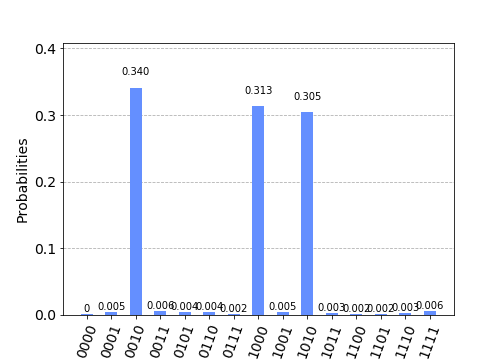
\includegraphics[scale=0.5]{NotebookHistogram}
						\caption{4-SAT solutions from the jupyter notebook}
					\end{figure}
				
					\item From the transpiled version we were able to retrieve that:
					\begin{verbatim}
					gates = OrderedDict([('cx', 523), 
					                     ('u3', 184), 
					                     ('u1', 102), 
					                     ('u2', 50), 
					                     ('measure', 4), 
					                     ('barrier', 2)])
					depth = 481
					\end{verbatim}
					The results make evidence of the fact that is not possible to realize physically a quantum device with 523 CNOT gates, 184 $U_3$ gates... The number of gates in fact is far above the limits regarding decoherence time of the current near-term quantum computer. This is another challenge that we managed in our implementation where we achieved an implementable circuit thanks to a simplified version of the problem.
				\end{enumerate} 
		
			\subsubsection{Decision Version}
			\label{sec:quantumDecisionVersion}
				In order to start the study of a quantum algorithm able to solve the SAT problem I continued after the description provided by qiskit, to consider several papers in which different conclusions where drawn. From these papers I noticed that two approaches are mainly considered to show the speedup achieved by running a quantum solver. As we may have guessed for this paper we decided to consider an implementation based on Grover' search because thanks to its step division we were able to fragment the code and focus better on each quantum principle that we have introduced in our study. However other approaches are possible, in particular some are based on the \emph{Quantum Fourier Transform} (QFT) algorithm able to show a different enhancement in terms of time complexity. \\
				
				The study of \cite[Ohya M. and Masuda N.]{quantumNP} considers this approach and provides also an example that allowed us to begin the implementation of a first complex quantum circuit able to store the instance of a general k-SAT implementation to be solved with the QFT algorithm. I used this paper as a toy example to begin working with qiskit and this approach led me to a very important conclusion that suggested once more that Grover's algorithm was the correct choice to face the problem. In particular the circuit that needs to be developed encodes the formulation of a k-SAT problem in a quantum device by using its formulation as a \emph{Conjunctive Normal Form}. To achieve the CNF we need to realize several AND and OR gates (as described in \ref{sec:operationsOnQubits}) and to bring the final superposition of the state encoded to a final qubit where the operations of the QFT algorithm are performed to find the solution. We are not now going deep on how this solution allows to show the improvement in terms of complexity (\cite[Ohya M. and Masuda N.]{quantumNP} shows the procedure) but we can use the circuit obtained to conclude a very important fact. As we have already described as one of the first issues of quantum devices we obtain a very high increasing of the number of qubits for some particular instances of a given problem. For the case of a k-SAT problem, with 3 variables we can already perceive this exponential growth, and the followings are the main reasons in this case:
				\begin{enumerate}
					\item The number of variables increases the OR operations to realize the disjunctive form of each clause. Each OR requires 3 qubits to be realized and an additional one to make the disjunction with the previous result.
					
					\item In the same way the number of clauses increases the AND operations to realize the conjunction of all the final disjunctive clauses.
					
					\item In addition the more clauses we have the more disjunctions and conjunctions we will need to realize
				\end{enumerate}
				Considering the formulation of \textbf{Problem 1} (\ref{sec:problem1}), we have a 3-SAT problem over 3 variables $x_1, x_2, x_3$; in order to encode the entire conjunctive normal form we need 20 ancillary qubits to perform the operations and an additional qubit to bring the final result of the conjunction (the method that allows to encode the clauses in the quantum circuit is present at \ref{c:decisionCircuit}) 
				\begin{figure}[h]
					\centering
					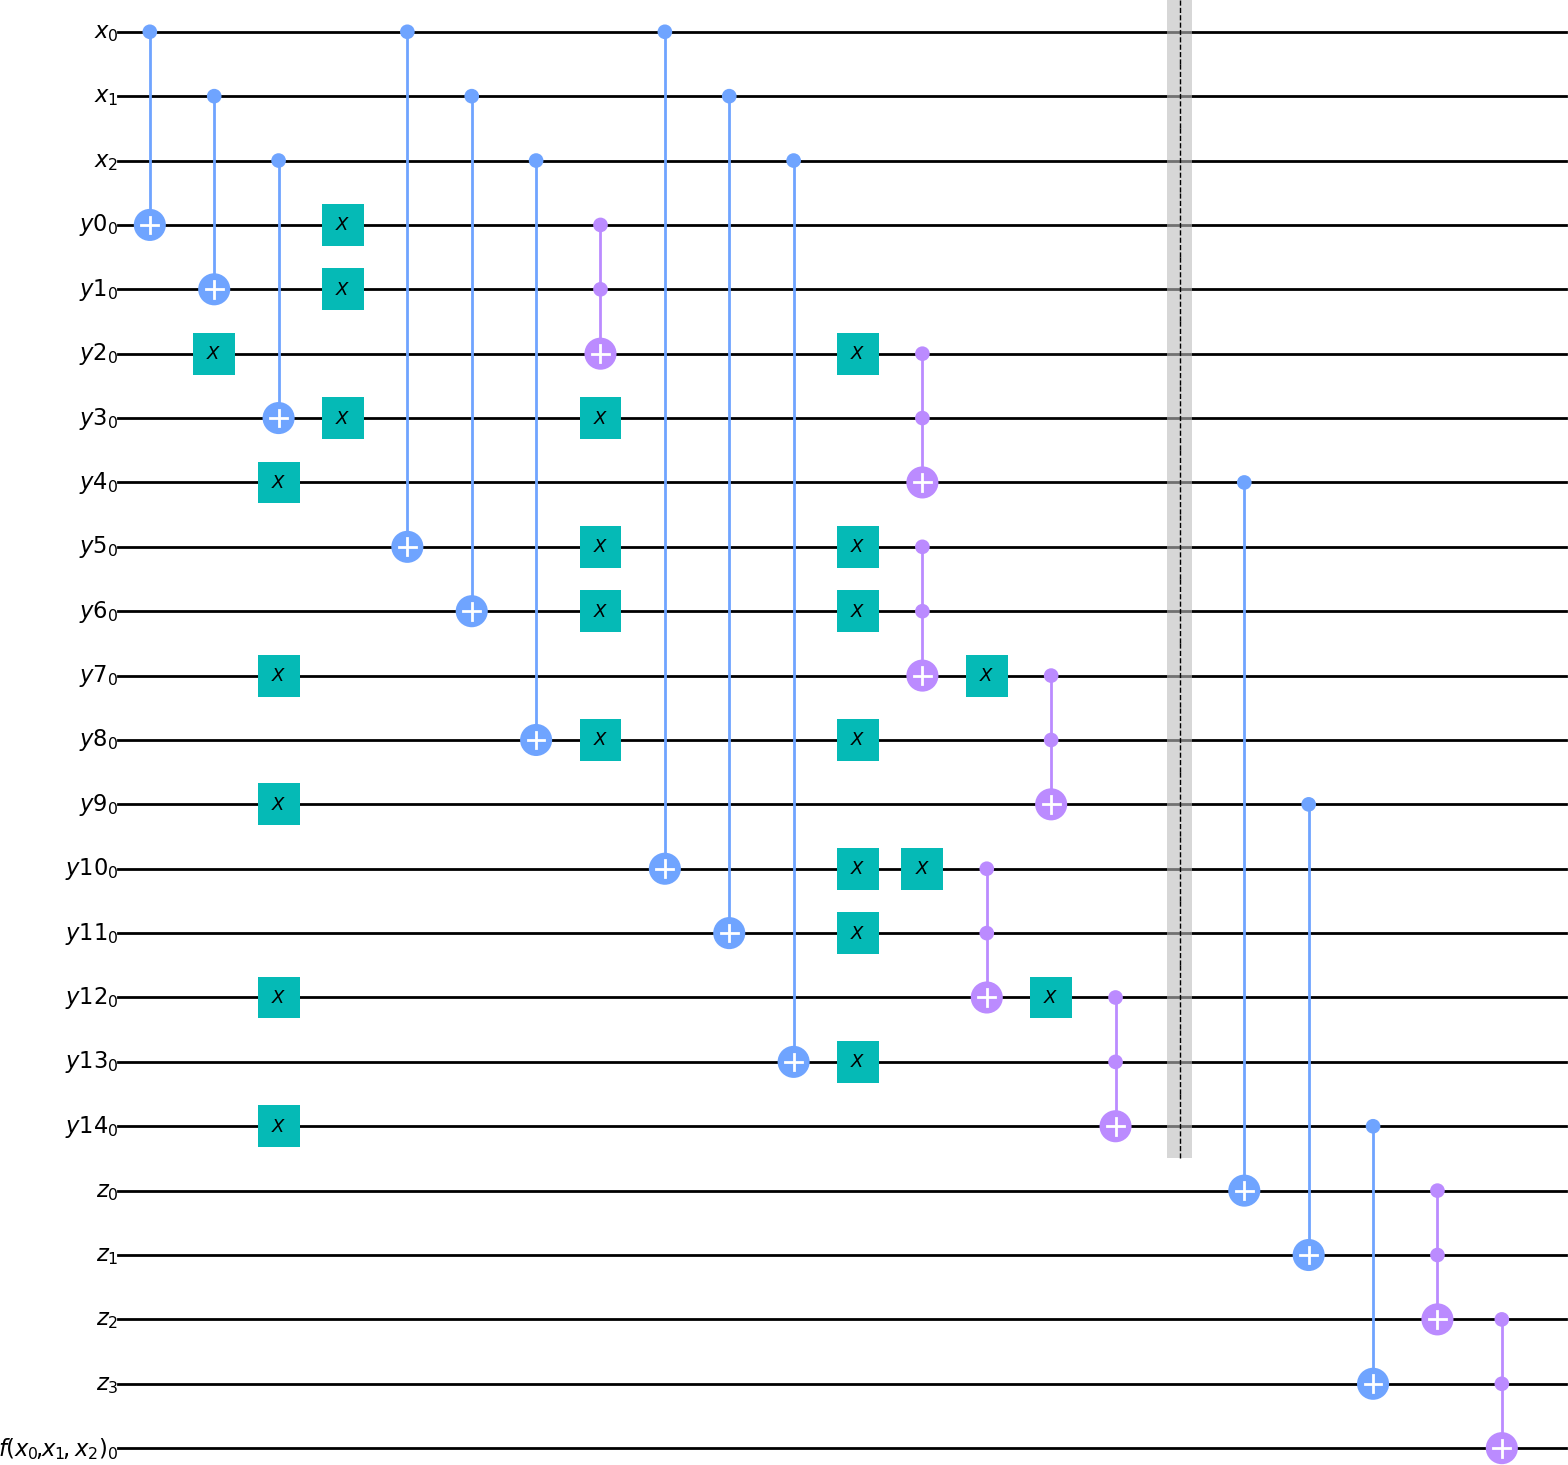
\includegraphics[scale=0.25]{DecisionCircuit}
					\caption{
						\label{fig:decisionVersionCircuit}
						Decision version circuit
					}
				\end{figure}
			
				Thanks to the observation for the exponential grow-up of the ancillary qubits needed to realize multiple gates in a circuit we understood that it was necessary to find a way to reuse the qubits. Considering the important no-cloning principle described in section \ref{conc:noCloning} we will se in the next section how we were able to realize a solver that uses less than 10 qubits in order to solve the exactly-1 problem for a 3-SAT problem, thus sticking with the decision of using Grover's search to solve an instance.
			
			\subsubsection{Exactly-1 k-SAT}
			\label{sec:quantumExactlyOne}
				We have finally arrived to the most complete implementation we developed for this paper in order to have an algorithm that was able to solve first a 3-SAT instance and then its generalization to the k-th case. Before describing how we implemented the steps of Grover's algorithm to solve the problem let's remark the definition of an exactly-1 k-SAT problem.
				
				\paragraph{Definition (Exactly-1 k-SAT):} \emph{Given a k-SAT problem we want to determine a satisfying assignment containing one true literal per clause.} \\
				
				This definition helps us to reduce the complexity in which a general k-SAT solver works (see qiskit's implementation at \ref{sec:quantumQiskitSolver}) and allows to realize an algorithm that performs iterations of Grover's algorithm to find the solutions. In the following we will describe precisely how the steps composing Grover's algorithm are implemented as the phenomenon of \emph{amplitude amplification} allows to modify the coefficients of the possible solutions for a given problem and find the best ones. \\
				
				As described in \cite[G.Nannicini, 2020]{introNoPh} three steps are needed to implement the solver, and the number of iterations of these steps is fundamental to find solutions that are significant. The following list describes precisely how we implemented the steps in the generalized version of a solver for a general exactly-1 k-SAT problem with an arbitrary number of clauses:
				\begin{enumerate}
					\item \textbf{Initialization:}\\
					Grover's algorithm applies to a function with an n-qubit input and a single qubit output. We call \texttt{f\_in} the input register of the encoded function $U_f$, of size n, and \texttt{f\_out} the output register of $U_f$, of size 1. The initialization of a quantum algorithm, as we have discussed in the conclusion \ref{conc:superposition}, consists of applying the Hadamard gate to the quantum state composed of n-qubits in order to obtain the uniform superposition to work with. Thus the piece of code that corresponds to the method:
				\end{enumerate}
				\vspace{-0.2cm}
				\begin{lstlisting}[]
                  def input_state(circuit, f_in, f_out):
				\end{lstlisting}
				\vspace{-0.3cm}
				\begin{figure}[h]
					\hspace{-1.9cm}Is equivalent to the following circuit:\vspace{0.2cm} \\
					\centering
					\mbox{
						\Qcircuit @C=1em @R=.7em {
							\lstick{\texttt{f\_in} \ket{0}_n} & \qw & \qw {/}^n & \gate{\otimes^n\mathcal{H}} & \qw {/}^n \\
							\lstick{\texttt{f\_out} \ket{0}_1} & \qw & \gate{X} & \gate{\mathcal{H}} & \qw
					}}
					\caption{Initialization step of Grover's algorithm}
				\end{figure}
				\begin{enumerate}[resume]
					\item \textbf{Black-box function $U_f$}:\\
					Implementing $U_f$ is the most complex part of the algorithm, in particular now that we want to generalize the case allowing the possibility to have more than 3 variables only. The problem of computing $U_f$ is in fact decomposed for each clause by introducing m auxiliary qubits, one per each clause. And for each clause we build a circuit that bit-flips the auxiliary qubit of the corresponding auxiliary qubit if and only if the clause has exactly one true literal. Finally, we apply a bit-flip on the output register of $U_f$ if and only if all m auxiliary qubits are 1. In figure \ref{fig:blackBoxCircuit} we can see the example of the circuit that we want to implement in order to flip the last qubit if the clause $x_1\lor \neg x_2\lor x_3 \lor \neg x_4$ is satisfied by exactly one literal. The circuit contains NOT gates to encode the negated variables and then to define the double implication of flipping $\ket{y}$ we first use 4 CNOTS to bring each qubit on the last one. Thus we now have $\ket{y} = \ket{y\oplus x_1 \oplus \neg x_2 \oplus x_3 \oplus \neg x_4}$, and the quadruply-controlled gate leads the auxiliary qubit of the clause to $\ket{y}= \ket{y\oplus x_1 \oplus \neg x_2 \oplus x_3 \oplus \neg x_4 \oplus (x_1\land \neg x_2 \land x_3 \land \neg x_4)}$. This sets $\ket{y} = \ket{1}$ if and only if exactly one literal is satisfied because as we know from the initialization of every new qubit we always have the starting value of $\ket{0}$. 
					\begin{figure}[ht]
						\centering
						\mbox{
							\Qcircuit @C=1em @R=.7em {
								\lstick{\ket{x_1}} & \qw & \ctrl{4} & \qw & \qw & \qw & \ctrl{4} & \qw & \qw \\
								\lstick{\ket{x_2}} & \gate{X} & \qw & \ctrl{3} & \qw & \qw & \ctrl{3} & \gate{X} & \qw \\
								\lstick{\ket{x_3}} & \qw & \qw & \qw & \ctrl{2} & \qw & \ctrl{2} & \qw & \qw \\
								\lstick{\ket{x_4}} & \gate{X} & \qw & \qw & \qw & \ctrl{1} & \ctrl{1} & \gate{X} & \qw \\
								\lstick{\ket{y}} & \qw & \targ & \targ & \targ & \targ & \targ & \qw & \qw
						}}
						\caption{
							\label{fig:blackBoxCircuit}
							Circuit for the clause $x_1\lor \neg x_2\lor x_3 \lor \neg x_4$
						}
					\end{figure}
				
					To implement this circuit in Qiskit there is a problem: only double controlled gates are implemented in the library. To overcome this issue we can easily concatenate CCNOT gates adding an ancillary qubit for each of the additional variables. In this way we will compute the partial results of the CCNOT between two variables and by storing this value in the first auxiliary qubit we continue with another CCNOT with the next variable. In the end we also perform another CCNOT with all the variables which targeted the auxiliary qubits to reset their state to the initial $\ket{0}$ and reuse them for the circuit of the following clauses. To understand better the mechanism of generalization we can see how the circuit is implemented in our algorithm in figure \ref{fig:generalizedBlackBoxCircuit}. In the circuit we represent how to realize a quadruply-controlled NOT gate with the reset of the auxiliary qubits initialized as $\ket{0}$. This fragment of the code is the one that substitutes the last gate that we can see above in the real implementation. As we can see we added two ancillary qubits $a_1$ and $a_2$ (initialized as $\ket{0}$) to "bring" the final result of the CNOT gate between the four variables $x_1, x_2, x_3, x_4$. 					
					\begin{figure}[ht]
						\centering
						\mbox{
							\Qcircuit @C=3em @R=1.1em {
								\lstick{\ket{x_1}} & \ctrl{4} & \qw & \qw & \qw & \ctrl{4} & \qw \\
								\lstick{\ket{x_2}} & \ctrl{3} & \qw & \qw & \qw & \ctrl{3} & \qw \\
								\lstick{\ket{x_3}} & \qw & \ctrl{3} & \qw & \ctrl{3} & \qw & \qw \\
								\lstick{\ket{x_4}} & \qw & \qw & \ctrl{3} & \qw & \qw & \qw \\
								\lstick{\ket{a_1}} & \targ & \ctrl{1} & \qw & \ctrl{1} & \targ & \qw \\
								\lstick{\ket{a_2}} & \qw & \targ & \ctrl{1} & \targ & \qw & \qw \\
								\lstick{\ket{y}} & \qw & \qw & \targ & \qw & \qw & \qw
						}}
						\caption{
							\label{fig:generalizedBlackBoxCircuit}
							Quadruply-controlled NOT gate
						}
					\end{figure}
					Finally we are able to implement the $U_f$ function trivially by looping over all the clauses and implementing for each of these the circuit of figure \ref{fig:blackBoxCircuit}, setting the auxiliary qubit \texttt{aux[k]} to 1 if clause $C_{k+1}$ is satisfied. In the end the method that allows to perform an iteration of the black-box function $U_f$ is:
				\end{enumerate}
				\vspace{-0.2cm}
				\begin{lstlisting}[]
def black_box_u_f(circuit, f_in, f_out, aux, n, exactly_1_k_sat_formula):
				\end{lstlisting}
				
				\begin{enumerate}[resume]
					\item \textbf{Inversion about the average:}\\
					The last operation we need to variate the coefficients of the possible quantum states of the solution is the inversion about the average. As precisely described in section \ref{sec:groverQuant} we can realize this operation with a unitary matrix that we called $W$. As we see from the definition (remember how to read the algebraic relation of a quantum circuit) we need first to perform Hadamard gates on the entire state, followed by the diagonal matrix $D$ and in the end negated Hadamard gates are performed once more on the entire quantum state. The implementation of $W$ is realized by the method:
					\begin{lstlisting}[]
def inversion_about_average(circuit, f_in, n):
      /* ... */
     def n_controlled_Z(circuit, controls, target):
     /* ... */
					\end{lstlisting}
					To generalize the $D$ matrix we need to implement a $C^{n-1}Z$ gate (realized by \texttt{n\_controlled\_Z} defined above). Also in this case for more than 2 controls we need to realize multiple controlled NOT gates. In fact to realize the gate we round the controlled NOT gate of all the controls passed as argument of the method \texttt{n\_controlled\_Z}, with two Hadamard gates. Considering how we dealt with the problem of multiply-controlled NOT gates we can see in figure \ref{fig:cZgate} how the diagonal matrix $D$ is implemented for the case of 4 control qubits. In the actual implementation also in this case we reset the state of the ancillary qubits as they will be reused at the next iteration of the amplitude amplification phase.
				\end{enumerate}
				\begin{figure}[ht]
					\hspace{0.3cm}
					\centering
					\mbox{
						\Qcircuit @C=2em @R=1.1em {
							\lstick{\ket{c_1}} & \qw & \ctrl{4} & \qw & \qw \\
							\lstick{\ket{c_2}} & \qw & \ctrl{3} & \qw & \qw \\
							\lstick{\ket{c_3}} & \qw & \ctrl{2} & \qw & \qw \\
							\lstick{\ket{c_4}} & \qw & \ctrl{1} & \qw & \qw \\
							\lstick{\ket{target}} & \gate{H} & \targ & \gate{H} & \qw
					}}
					\caption{
						\label{fig:cZgate}
						Theoretical $C^{n-1}Z$ gate
					}
				\end{figure}
				\newpage
				Now that we have the complete implementation of all the steps that compose the amplitude amplification in grover's algorithm we have to choose how many time to iterate them in order to solve the problem. As it is done in \cite[G.Nannicini, 2020]{introNoPh} we decided to do the same by iterating twice the bit-flip and the inversion about the average steps. As we can see in the actual implementation, once the problem has been encoded in the quantum circuit we run the \texttt{grover} method in order to solve the instance. The definition of Grover's algorithm with two iterations is the following:
				\begin{lstlisting}[]
def grover(self):
    self.__input_state()
    self.__black_box_u_f()
    self.__inversion_about_average()
    self.__black_box_u_f()
    self.__inversion_about_average()
				\end{lstlisting}
				
			\subsubsection{Significant Results}
			\label{sec:quantumResults}
				The results we obtained from the execution of the quantum solver for the generalized exactly-1 k-SAT problem will show how we were able to solve the four problems formalized before (\ref{sec:satInstances}) with the three steps of the Grover's search algorithm that we have studied, thus obtaining the quadratic speedup provided by this quantum algorithm. We will start by focusing on showing the correct execution of the solver by proving the consistency of the results that we obtained from the counts of the quantum experiments run to solve each instance. Then, we will continue with a step by step description of how \textbf{Problem 3} is encoded in the quantum circuit, to show how we managed to implement the generalized version of the solver, in the case of a number of clauses and length greater than 3. The solutions that we have obtained for each of the problems are now listed:
				\begin{itemize}
					\item \textbf{Problem 1:} \\
						As we can see from the formulation of the first problem (\ref{sec:problem1}), there is one only solution for the exactly-1 3-SAT problem that is: $S=\{x_1, \neg x_2, x_3\}$. Executing our solver we obtained the solution shown in the following picture (\ref{fig:problem1Solution}):
						\begin{figure}[h]
							\centering
							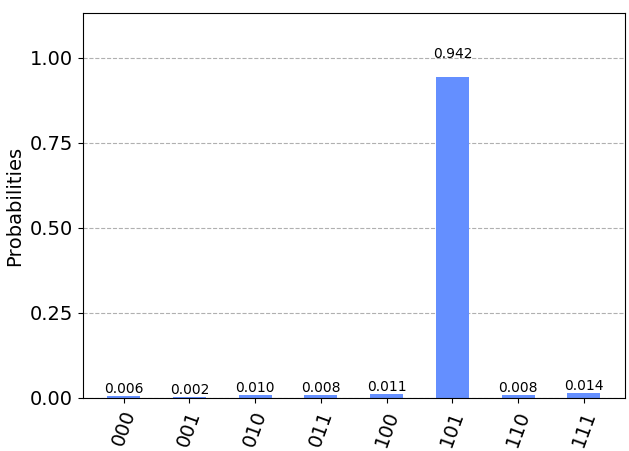
\includegraphics[scale=0.35]{Problem_1_Solution.png}
							\caption{
								\label{fig:problem1Solution}
								Solution of the exactly-1 Problem 1 
							}
						\end{figure}
					
						As we can see from the picture above the result is the string $101$, representing the solution $S$ provided before, with a probability near the $95\%$ which is a very nice result mitigated by the fact that the quantum device on which the algorithm has been run is the \texttt{qasm\_simulator} provided by the Aer package of qiskit.
					
					\item \textbf{Problem 2:} \\
						As we can see from the formulation of the second problem (\ref{sec:problem2}), the simplest solution of the exactly-1 3-SAT problem can be grasped from its simple structure: $S=\{x_1, x_2, x_3, x_4, x_5\}$.  Executing our solver we obtained the solution shown in the following picture (\ref{fig:problem2Solution}):
						\begin{figure}[h]
							\centering
							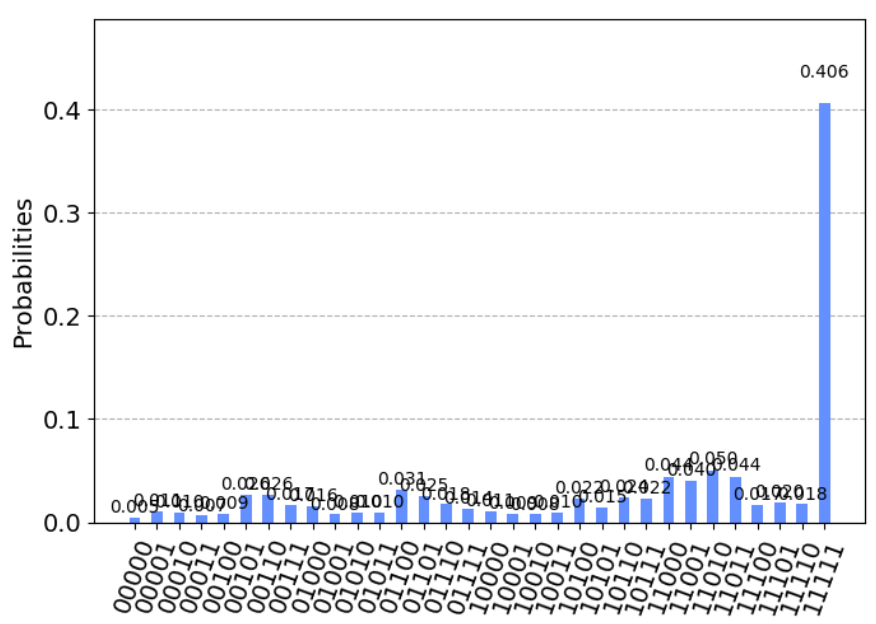
\includegraphics[scale=0.7]{Problem_2_Solution.png}
							\caption{
								\label{fig:problem2Solution}
								Solution of the exactly-1 Problem 2
							}
						\end{figure}
					
						As we can see from the picture above the result is the string $11111$, representing the solution $S$ provided before, with a probability near the $40\%$ significantly higher than all the other 5 qubits combinations. As always we have to remember that these simulations have been run on a quantum simulator that is much less noisy than its real correspondent device.
					
					\item \textbf{Problem 3:} \\
						As we can see from the formulation of the third problem (\ref{sec:problem3}) and from the results of the execution of the classical solver, the problem is trivially satisfiable for example with $S = \{\neg x_1, x_2, \neg x_3\}$. But this one is not a solution for the exactly-1 formulation of this problem, in fact we can see that in the second clause both $\neg x_1$ and $\neg x_3$ make the disjunction true. The exactly-1 Problem 3 has no solutions and the result we obtained from the execution of our solver is shown in figure \ref{fig:problem3Solution}:
						\begin{figure}[h]
							\centering
							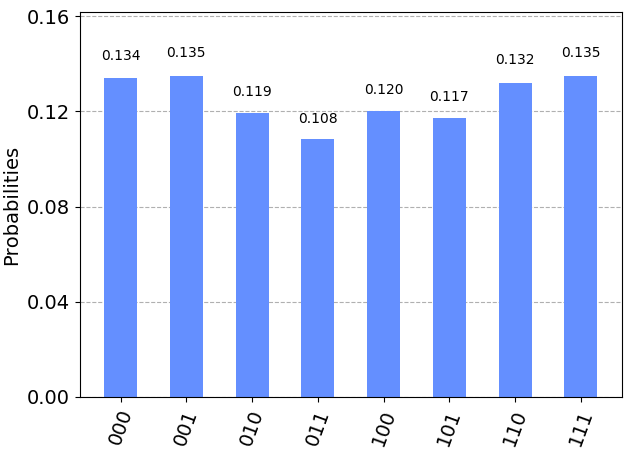
\includegraphics[scale=0.41]{Problem_3_Solution.png}
							\caption{
								\label{fig:problem3Solution}
								Solution of the exactly-1 Problem 3
							}
						\end{figure}
					
						As we can see from the picture above none of the possible strings can be considered with respect to the others. The probability rounds over the $10\%$ for each possibility and this does not allow to choose one string among the others. However, knowing that the problem is satisfiable we can use the implementation of the most general solver provided by Qiskit (shown in the jupyter notebook at \ref{sec:quantumQiskitSolver}) to prove the consistency of the result also with a quantum solver.
						
					\item \textbf{Problem 4:} \\
						As we can see from the formulation of the fourth problem (\ref{sec:problem4}), the trivial solution of this 4 variables and 4 clauses exactly-1 4-SAT problem is $S=\{x_1, x_2, x_3, x_4\}$. This problem has been used to show the correct working of the solver that generalizes the problem of an exactly-1 k-SAT problem with an arbitrary number of clauses. Executing our solver we obtained the solution shown in the following picture (\ref{fig:problem4Solution}):
						\begin{figure}[h]
							\centering
							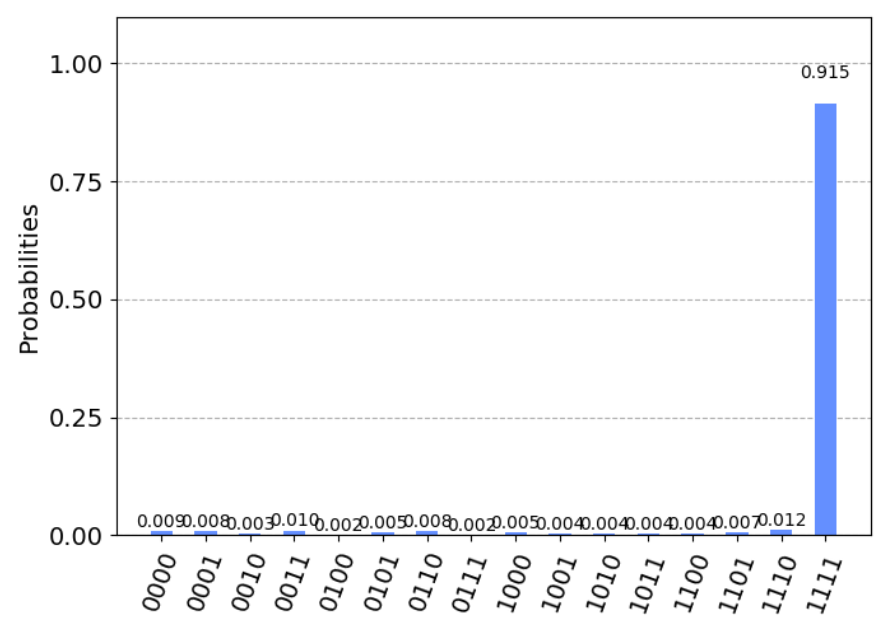
\includegraphics[scale=0.42]{Problem_4_Solution.png}
							\caption{
								\label{fig:problem4Solution}
								Solution of the exactly-1 Problem 4
							}
						\end{figure}
					
						As we can see from the picture above the result is the string $1111$, representing the solution $S$ provided before, with a probability near the $90\%$ significantly higher than all the other probabilities. 
				\end{itemize}
				Now that we have shown how the implementation of the exactly-1 solver is able to provide the correct solutions even for the generalized formulation where more than 3 variables are present in a single clause, it is important to show how is shaped the circuit that allows us to find the solution. In order to show how the generalization of each of the three steps of Grover's search is implemented in the circuit, considering \textbf{Problem 4} we can now see how each of the step is reflected in the actual circuit that is run on the quantum device. As we have precisely described in the implementation of the exactly-1 k-SAT problem (section \ref{sec:quantumExactlyOne}) the three steps are:
				\begin{enumerate}
					\item \textbf{Initialization:}\\
						The first thing we need to do in order to build the quantum circuit is to bring the state composed of the 4 qubits representing the four variables in a uniform superposition. In order to do so we consider an additional qubit and apply on the first four the Hadamard gate while on the additional one we apply in sequence an X gate followed by another Hadamard. The result of the initialization step for the exactly-1 \textbf{Problem 4} is shown in the following figure (\ref{fig:initializationCircuit}):
						\begin{figure}[h]
							\centering
							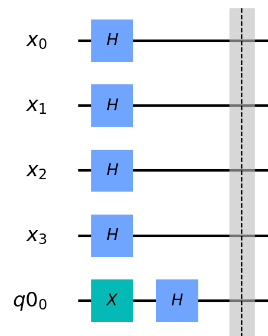
\includegraphics[scale=0.8]{Initialization_Circuit.png}
							\caption{
								\label{fig:initializationCircuit}
								Initialization fragment in Problem 4 circuit
							}
						\end{figure}
					
					\item \textbf{Clause Encoding \& Black Box $U_f$:}\\
						The second step encodes the black box function $U_f$ for each of the clauses that the SAT problem is composed of. Hence with four clauses we will have four similar parts in the circuit each encoding one of the different clauses. To understand how this process is reflected in the circuit we now consider the clause $C_1 = \{x_1, \neg x_2, \neg x_3, \neg x_4\}$ as we can see how the circuit is generalized also for the case of a length greater than 3. As we can see in picture \ref{fig:clauseEncodingCircuit}, each clause is delimited by two barriers in the actual circuit as they can be easier to be identified. Starting from the first part we see how the variables are brought to the first ancillary qubit needed to bring the positive result in case one and one only literal is true in the clause. Once each variable is carried on the ancillary qubit with the respective polarity we need to perform a quadruply-controlled NOT gate of all the four variables and bring this result on the ancillary qubit. To do so, as we described in the black box step in section \ref{sec:quantumExactlyOne}, we will use a sequence of CCNOT gates with additional ancillary qubits to carry the partial results. This phase is visible at the centre of the circuit where first the result is brought on the first ancillary qubit $q1_0$ and then additional CCNOT gates are used to reset the ancillary qubits used for the following clauses. In the end also the variables are reset to the initial superposition as they can be reused for the following clauses.
						\begin{figure}[h]
							\centering
							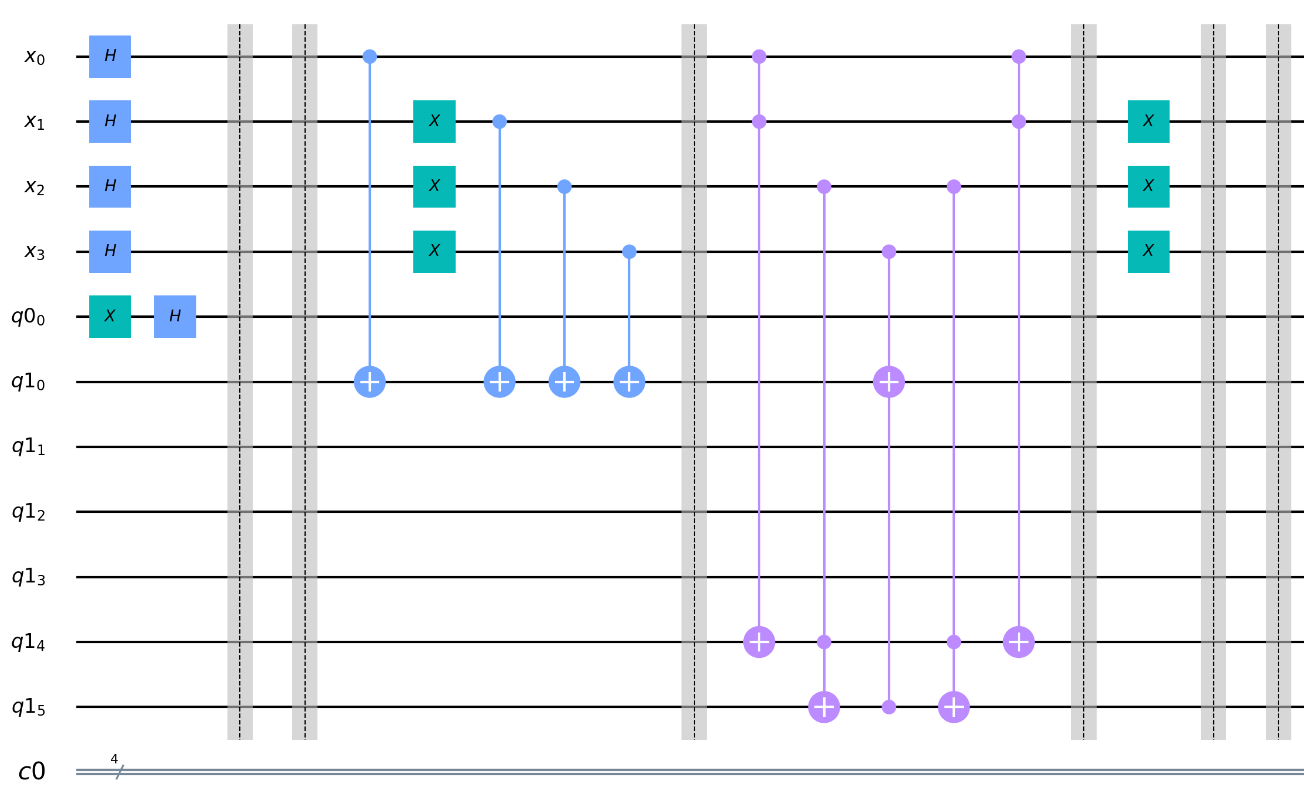
\includegraphics[scale=0.55]{Clause_Encoding_Circuit.png}
							\caption{
								\label{fig:clauseEncodingCircuit}
								Clause encoding and black box $U_f$ in Problem 4 circuit
							}
						\end{figure}
					
					\item \textbf{Inversion About the Average:}\\
						The last step before the four qubits can be measured in order to find the solution of the problem is the inversion about the average; achieved with the unitary matrix $W = (-\otimes^n\mathcal{H})D(\otimes^n\mathcal{H})$. As we have described in the implementation section also in this case, between the Hadamard gates we need to realize a multiply-controlled NOT gate. In the case of 4 variables the $C^{n-1}Z$ gate has size 3 hence we will realize the triply-controlled NOT gate as we have already described and in the end, after the additional Hadamard gates we will measure the four qubits corresponding to the four variables of the problem to find the solution.
						\begin{figure}[h]
							\centering
							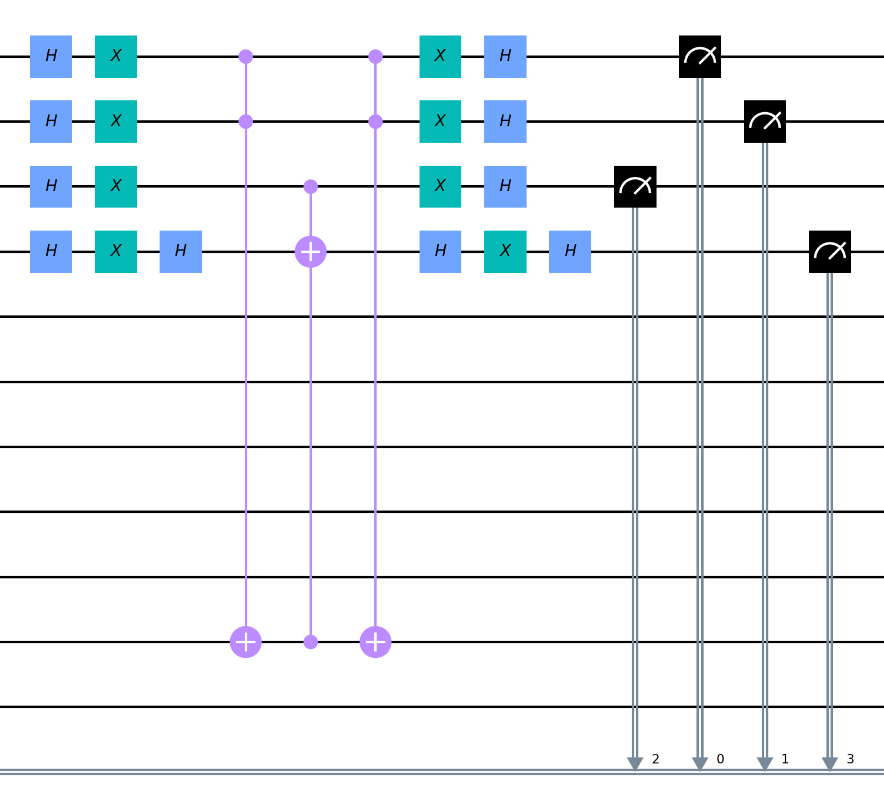
\includegraphics[scale=0.67]{Average_Inversion_Circuit.png}
							\caption{
								\label{fig:averageInversionCircuit}
								Inversion about the average in Problem 4 circuit
							}
						\end{figure}
				\end{enumerate}
			
		\subsection{Classical vs. Quantum}
		\label{sec:satCsatQ}
			We are finally arrived to the actual comparison between the algorithms able to solve the k-SAT problem that we have used to complete the study of the quantum world. Now that we have described each of the implementations to solve this problem we are able to define the comparison in terms of the peculiarities highlighted so far for each algorithm. To compare the classical and the quantum versions of the solvers, in this section we will depict for each feature a separate study in order to understand better the advantages and disadvantages of the two possible solutions.
			
			\subsubsection{Complexity}
			\label{sec:complexityComparison}
				In terms of complexity we have always to refer to the two different types of complexity we described in \ref{sec:algorithmComplexity}. As we have said we mainly focused on time complexity but we were still able to see that in the quantum algorithms it is still an issue, for some problems, the exponential growth of the qubits needed to realize the circuit encoding the algorithm. In the case of the SAT for the classical case we were able to exploit a very efficient way to encode the problems while as we saw for the case of the \emph{decision version} implementation (\ref{sec:quantumDecisionVersion}), ancillary qubits may grow very fast when several operations are needed. In the \emph{exactly-1} implementation instead we were able to reset some of the additional qubits needed as they may be reused; however we have always to keep in mind the \textbf{no-cloning} principle which tells that to obtain the same state of a quantum device we have no other solution than to repeat the same operations from the initial state. \\
				
				Talking about time complexity, also in this case we saw that it can be faced in two different ways depending on the algorithm we use to solve our problem. In the \emph{decision version} with the QFT algorithm we would be able to make the comparison in terms of number of elementary operations as we are used to do. Unfortunately this discussion is much more difficult both in terms of quantum physical theory and for the space complexity issue depicted above, that made us focus on the other definition. By using Grover's search algorithm, in fact, we were able to describe more precisely all the fundamentals we introduced at the beginning of the paper in the steps that compose the algorithm. In this way the implementation shows directly in the quantum circuit how the algorithm is executed and allows to understand better how the solution is found. In terms of complexity, being Grover a search algorithm we have considered the so called \textbf{query complexity}, that allowed us to compare the results obtained with those present in classical algorithms. We have listed the complexities of the most efficient classical algorithms in \ref{sec:satClassical} to understand how close we are to have algorithms that can solve $\mathcal{N}\mathcal{P}$-complete in almost a non-exponential time complexity. Grover's search allows to solve these algorithms based on the search of the solution for the k-SAT problem defined with a quadratic speedup and this is the most important conclusion we can derive from this comparison. \\
				
				The comparison between the different algorithms leads also to consider that quantum algorithms are based on probability theory that describes the quantum state of the quantum algorithm while the execution is running. In the same way randomized classical algorithms are focussing on probability aspects that may be merged in the quantum algorithms in order to find other algorithms, not necessarily focusing on the search of the solution, but exploiting probability and physics aspects that combined together can bring a solution. This is a completely different way of studying algorithms, and it shows how it is fundamental first to understand the concepts of the nature behind the algorithm before realizing the quantum circuit to be executed. 
			
			\subsubsection{Implementation}
			\label{sec:implementationComparison}
				It is also important to compare how a classical algorithm is implemented with respect to its quantum counterpart, in particular for the conclusion we have just derived in the previous feature. As we may have grasped there is not a complete correspondence between a classical and a quantum algorithm. In fact we are so used to implement classical algorithms that we tend to consider quantum ones as steps corresponding to the classical version but encoded on a quantum circuit. This is not completely true, for what we said before, but it is the direction that this study is following for the extremely large amount of studies that have been developed on classical algorithms so far. As we can see in the case of the k-SAT problem, in the classical case we used a backtracking technique on a the search tree to find the solution. In the same way in the quantum implementations we used Grover's search to look for the solution. \\
				
				This aspect is both an advantage and a drawback for the study of quantum computing: from one perspective, in fact, we have working algorithms that can be reused for different problems thus bringing the enhancements of that implementation; on the other hand we are not sure that the algorithm we are realizing is the best way to find a solution for the problem in a quantum world. 
				
			\subsubsection{General View}
			\label{sec:generalViewComparison}
				From a general point of view we can say that quantum algorithms seem to provide actually the speedup promised. To draw a real comparison in terms of execution time and space occupied during an execution it is still difficult to find significant results both for the different time complexities to be considered and for the different kind of memory that the classical and quantum devices are based on. As we have studied in the papers that are cited in this study, in fact, the complexity study approach is always theoretical but with solid mathematical proofs that show how the speedup is actually achieved; in particular with Grover's algorithm that we decided to use the enhancement with respect to the classical search is quadratic. 
			
	\section{Conclusions}
	\label{sec:conclusions}
		The important conceptual conclusions we wanted to highlight in this paper have already been precisely identified during the study thanks to their formal definitions in the paragraphs that we called \textbf{Conclusion i}. Taking care of their importance for the study of the algorithm we decided to use as the coding reference for this work we want now to focus on the conclusions that we were able to understand thanks to the final comparison of the previous section, by showing in a complete and resuming way how the actual quadratic speedup is achieved by using Grover's search algorithm. \\
		
		Starting from the beginning we first understood how important is to have clear in mind the physical principles behind the \emph{state of the art} of quantum computation before starting to define quantum algorithms. Once the fundamentals were described we were able to formally define a quantum device to have a strong comparison with the classical case once we began to encode an algorithm inside a quantum circuit. The first conclusion identified while describing a quantum algorithm is the exponential growth of the qubits to encode an algorithm and the \emph{superposition} and \emph{entanglement} principles on which almost every quantum algorithm is based on. For the problem of the number of qubits we also studied the \emph{no-cloning} principle which obliged us to design algorithms in such a way to reuse ancillary qubits by resetting their state in order to keep control on the exponential growth. The main argument that we wanted to define was the speedup that quantum algorithms allow to achieve with respect to their classical counterparts. To do so we introduced the fundamentals of computational theory needed to understand how to compare a classical and a quantum algorithm and to see an implementation in action we used the k-SAT problem to show the different solvers. Studying Grover's search algorithm to implement a quantum solver we were able to go through the concepts studied in the paper and show with respect the classical algorithms complexities how a \textbf{quadratic} speedup can be obtained thanks to the three steps on which Grover is defined. \\
		
		In the end we have to remember that the entire paper is based on the use of Qiskit library which provides the advantages described in the respective section (\ref{sec:qiskit}), but several other libraries allow to define algorithms that can be run on quantum machines. Some examples are: Rigetti, Amazon Braket, Quantum Development Kit (Microsoft), Qsharp... Each of these solutions can be used for particular cases, once more we decided to stick with Qiskit for its wide development and simplicity for a first quantum approach. Finally, we have also understood that quantum algorithms have to be studied in a way that we are not still used to, focussing on the physical and mathematical aspects of the problem that we want to solve. For now, we computer scientist, can continue to study the algorithms that have already been studied and verified for the general problems and reuse them for the specific case we want to study, for example the SAT that we have considered in this paper. 
		
	\clearpage
	\begin{appendices}
		\section{Qiskit}
		\label{sec:qiskit}
			Qiskit is an open-source quantum computing software development framework for leveraging today's quantum processors. In the literature we find several different frameworks that allow to work with quantum computers, characterized by different implementation languages but from the quantum algorithm designer point of view, with different interfaces to the quantum computers and different simulators. In this paper I decided to use Qiskit because it is the most spread one, with a very good documentation and a wide community that updates every day the issues. Moreover, being realized by IBM it provides an experience called \emph{IBM quantum experience}(IBMQ) which allows to run the algorithms directly on a real quantum computer rather than on a simulator. Qiskit is realized in python and this may suffice to explain why it has been chosen among the other solutions$\cdots$\\
			
			Thanks to its textbook \cite{qiskitTextbook} it provides a very wide and complete description on how to approach the area of quantum computing. Starting from the introductory subjects needed to face the basic principles of quantum physics it increasingly introduces how the library realizes the quantum operations that a user can define to implement its algorithms. Several examples are provided with jupyter notebooks where each step can be analysed in detail understanding how and what each instruction from the library does. I completely went through the entire notebook for my first approach to quantum computing and there I found the example I was looking for to produce this paper which is meant to simplify even more the introduction to this area, using a concrete example decomposed in different steps each introducing a particular aspect of how to use the library. Thanks to this notebook I realised the notebook visible in the repository at \textsc{Code/Quantum/quantumSat.ipynb} where I replicated the solution of the SAT problem by using the Grover solver implemented in the library. Thanks to the quantumSat.ipynb notebook I understood how difficult it is to realize the real implementation of a solver, interfacing directly with the quantum device, this helped me a lot to find a good way to realize an implementation of the same algorithm in a simpler case to solve the SAT problem. All the notes and some additional examples I realized during this first approach are present in the notebook. \\
			
			In conclusion it is very important to remark that Qiskit is an open source software where a great community is very available to help whoever wants to start studying quantum computing. Very interesting videos were also realized to give a further way to approach the library, thanks to them I learnt how to become a contributor of an open-source project and I became a contributor by solving an issue that can be visible at the following url: \url{https://github.com/Qiskit/qiskit-terra/pull/3751}.
		
		\section{Code with Qiskit}
		This section contains the list of the snippets of code needed to represent the examples used in the paper. To replicate them consider to import the following libraries:
		\lstinputlisting[language=python]{code/imports.py}
		
		\label{sec:codeWithQiskit}
			\begin{enumerate}
				\item \label{c:example3} \lstinputlisting[language=python]{code/example3.py}
				
				\item \label{c:example6} \lstinputlisting[language=python]{code/example6.py}
				
				\item \label{c:decisionCircuit} \lstinputlisting[language=python]{code/decisionSolver.py}
			\end{enumerate}
	\end{appendices}
	
	\clearpage
	\bibliographystyle{plain}
	\nocite{*}
	\bibliography{main.bib}
\end{document}

